%%%%%%%%%%%%%%%%%%%%%%% file template.tex %%%%%%%%%%%%%%%%%%%%%%%%%
%
% This is a general template file for the LaTeX package SVJour3
% for Springer journals.          Springer Heidelberg 2010/09/16
%
% Copy it to a new file with a new name and use it as the basis
% for your article. Delete % signs as needed.
%
% This template includes a few options for different layouts and
% content for various journals. Please consult a previous issue of
% your journal as needed.
%
%%%%%%%%%%%%%%%%%%%%%%%%%%%%%%%%%%%%%%%%%%%%%%%%%%%%%%%%%%%%%%%%%%%
%
% First comes an example EPS file -- just ignore it and
% proceed on the \documentclass line
% your LaTeX will extract the file if required
\begin{filecontents*}{example.eps}
%!PS-Adobe-3.0 EPSF-3.0
%%BoundingBox: 19 19 221 221view
%%CreationDate: Mon Sep 29 1997
%%Creator: programmed by hand (JK)
%%EndComments
gsave
newpath
  20 20 moveto
  20 220 lineto
  220 220 lineto
  220 20 lineto
closepath
2 setlinewidth
gsave
  .4 setgray fill
grestore
stroke
grestore
\end{filecontents*}
%
\RequirePackage{fix-cm}
%
%\documentclass{svjour3}                     % onecolumn (standard format)
%\documentclass[smallcondensed]{svjour3}     % onecolumn (ditto)
%\documentclass[smallextended]{svjour3}       % onecolumn (second format)
\documentclass[twocolumn]{svjour3}          % twocolumn
%
\smartqed  % flush right qed marks, e.g. at end of proof
%
\usepackage{graphicx}
%
% \usepackage{mathptmx}      % use Times fonts if available on your TeX system
%
% insert here the call for the packages your document requires
%\usepackage{latexsym}
% etc.
\usepackage{amsmath}
\usepackage{siunitx} %bh for reporting small p-values
\usepackage[authoryear]{natbib}
%
% please place your own definitions here and don't use \def but
% \newcommand{}{}
\long\def\comment#1{} %%% to comment out a section
%en added:
\usepackage{xspace}
\newcommand{\ie}[0]{{\em i.e.}\xspace}
\newcommand{\eg}[0]{{\em e.g.}\xspace}
\newcommand{\etal}[0]{{\em et al.}\xspace}
\newcommand{\etc}[0]{{\em etc.}\xspace}
\newcommand{\vs}[0]{{\em vs.}\xspace}
%\newcommand{\vv}[0]{{\em vice-versa}\xspace} % bh conflicts with esvect
\newcommand{\via}[0]{{\em via}\xspace}
\newcommand{\ibid}[0]{{\em ibid}\xspace}

\usepackage[h]{esvect} % for vector arrows, defined by \vv

%bh comment this out if we want to use esvect package
\renewcommand\vv{\overrightarrow}

%
% Insert the name of "your journal" with
\journalname{Journal of Computational Neuroscience}
%
\begin{document}

\title{A recurrent neural model for proto-object based contour integration and figure-ground segregation
\thanks{
% Remember to remove Pedja's grant!!!
This work is supported by
%the Office of Naval Research under 
%Grant N00014-15-1-2256 
%and 
the National Institutes of Health under Grants
R01EY027544 and R01DA040990.
}}
%\subtitle{Do you have a subtitle?\\ If so, write it here}

%\titlerunning{Short form of title}        % if too long for running head

\author{Brian Hu        \and
        Ernst Niebur %etc.
}

%\authorrunning{Short form of author list} % if too long for running head

\institute{
           Brian Hu \at Zanvyl Krieger Mind/Brain Institute and
           Department of Biomedical Engineering,  Johns Hopkins University, Baltimore, MD 21218, USA \\
           Tel.: +1 410 516-8640\\
           Fax.: +1 410 516-8648\\
           \email{bhu6@jhmi.edu}           \\
\and Ernst Niebur \at  Zanvyl Krieger Mind/Brain Institute and
           Solomon Snyder Department of Neuroscience,  Johns Hopkins
           University, Baltimore, MD 21218, USA \\
\email{niebur@jhu.edu}}

\date{Received: date / Accepted: date}
% The correct dates will be entered by the editor


\maketitle

\begin{abstract}
Visual processing of objects makes use of both feedforward and
feedback streams of information.  However, the nature of feedback
signals is largely unknown, as is the identity of the neuronal
populations in lower visual areas that receive them.
Here, we develop a recurrent neural model to address these questions
in the context of contour integration and figure-ground segregation. 
A key feature of our model is the use of 
{\em grouping neurons}
 whose activity represents 
tentative objects (``proto-objects'')
based on the integration of local feature information. Grouping
neurons receive input from an organized set of local feature neurons, and project
modulatory feedback to those same neurons. 
Additionally, inhibition at both the local feature level and the
object representation level biases the interpretation of the visual scene
in agreement with principles from Gestalt psychology.
Our model explains several sets of neurophysiological
results~\citep{Zhou_etal00,Qiu_etal07,Chen_etal14},
and makes testable predictions about the influence of 
neuronal feedback and attentional selection
on neural responses across different visual areas.  Our
model also provides a framework for understanding how object-based
attention is able to select both objects and the features associated
with them.  
\keywords{recurrent processing \and shape perception \and
  feedback, grouping \and perceptual organization \and contour
  processing}
% \PACS{PACS code1 \and PACS code2 \and more}
% \subclass{MSC code1 \and MSC code2 \and more}
\end{abstract}

\section{Introduction}
\label{intro}

Gestalt psychologists recognized the importance of the whole in
influencing perception of the parts when they laid out several
principles (``Gestalt laws'') for perceptual
organization~\citep{Wertheimer23,Koffka35}. Contour integration, the
linking of line segments into contours, and figure-ground segregation,
the segmenting of objects from background, are fundamental components
of this process. Both require combining local, low-level and global,
high-level information
that is represented in different areas of the brain
in order to segment the visual scene. The interaction between feedforward and
feedback streams carrying this information, as well as the
contribution of top-down influences such as 
attentional selection, 
are not well understood. 

The contour integration process begins in primary visual cortex (V1),
where the responses of orientation selective neurons can be modulated
by placing collinear stimuli outside the receptive fields (RFs) of
these neurons~\citep{Stemmler_etal95a,Polat_etal98}.  Contextual
interactions between V1 neurons have often been summarized using a
``local association field,'' where collinear contour elements excite
each other and noncollinear elements inhibit each other
\citep{Ullman92, Field_etal93}.  Results from neuroanatomy lend
support to these ideas, as the lateral connections within V1
predominantly link similar-orientation cortical columns
\citep{Gilbert_Wiesel89,Bosking_etal97,
  Stettler_etal02}. Computational models based on these types of local
interactions have successfully explained the ability of V1 neurons to
extract contours from complex
backgrounds~\citep{Li98,Yen_Finkel98,Piech_etal13}. While some of
these models also incorporate feedback
connections, the mechanisms by which higher visual areas construct the
appropriate feedback signals and target early feature neurons are not
clearly specified.  One of the main purposes of the present study is
to introduce concrete neural circuitry that makes this recurrent
structure explicit, thereby allowing us to make quantitative
predictions and compare model predictions with experimental data.

Segmenting an image into regions corresponding to objects requires not only finding the contours in the image but also determining which contours belong to which objects.
This is part of what is known as the {\em binding problem,} as it is unclear how higher visual areas ``know'' which features belong to an object~\citep{Treisman96b}.
One solution involves differential
neural activity, where the neurons responding to the features of an
object show increased firing compared with neurons responding to the
background.  Such response enhancement was first observed in V1 for texture-defined
figures~\citep{Lamme95}. Alternatively, it has been proposed that
binding is implemented by neurons that represent features of the same
object firing in synchrony while neurons representing features of
different objects firing asynchronously \cite[``binding by
synchrony;'' for review see][]{Singer99b}. While this is an attractive
and parsimonious hypothesis, experimental evidence is
controversial~\citep{Gray_etal89,Kreiter_Singer92,DeOliveira_etal97,Thiele_Stoner03,Roelfsema_etal04,Dong_etal08a}.

Border-ownership selective cells that have been found in early visual
areas, predominantly in secondary visual cortex (V2), appear to be
dedicated to this task~\citep{Zhou_etal00}.  Border-ownership
selective cells encode where an object is located relative to their
RFs.  When the edge of a figure is presented in its RF, a
border-ownership cell will respond with different firing rates
depending on where the figure is located.  For example, a vertical
edge can belong either to an object on the left or on the right of the
RF. A border-ownership selective cell will respond differently to
these two cases, firing at a higher rate when the figure is located on
its ``preferred'' side, even though the stimulus within its RF may be
identical. For a more detailed operational definition of how
border-ownership selectivity is determined experimentally, see
Section~\ref{sec:FGO}. Border-ownership coding has been studied using
a wide variety of artificial stimuli, including those defined by
luminance contrast, color contrast, figure outlines ~\citep{Zhou_etal00}, 
motion~\citep{vonderHeydt_etal03a},
disparity~\citep{Zhou_etal00,Qiu_vonderHeydt05}, and
transparency~\citep{Qiu_vonderHeydt07} as well as, more recently, with
faces \citep{Hesse_Tsao16} and within complex natural scenes
\citep{Williford_vonderHeydt14}.

To explain this phenomenon, some computational models assume that
image context integration is achieved by propagation of neural
activity along horizontal connections within early visual
areas. Border-ownership information could be generated from the 
asymmetric organization of surrounds \citep{Nishimura_Sakai04,
 Nishimura_Sakai05,Sakai_etal12} or from a diffusion-like process
within the image representation~\citep{Grossberg94,Grossberg97,
Baek_Sajda05, Kikuchi_Akashi01, Pao_etal99,
Zhaoping05}. However, these models have difficulties explaining the
fast establishment of border ownership which appears about 25ms after
the first stimulus response \citep{Zhou_etal00}.
 Propagation along horizontal fibers over the
distances used in the experiments would imply a delay of at least $\approx70$ms \citep[][based on the conduction velocity of horizontal fibers in primate V1 cortex; we are not aware of corresponding data for V2]{Girard_etal01}. Furthermore, such models are difficult to reconcile with the observation that the time course of border-ownership coding is largely independent of figure size~\citep{Sugihara_etal11}.

An alternative computational model involves populations of grouping
(G) cells which explicitly represent (in their firing rates) the
perceptual organization of the visual scene~\citep{Schutze_etal03,Craft_etal07}. 
These cells are reciprocally connected to
border-ownership selective (B) neurons through feedforward and
feedback connections.  The combination of grouping cells and the cells
signaling local features represents the presence of a ``proto-object''
\citep{Rensink00a},
resulting in a structured perceptual
organization of the scene. Among the operations that can be performed
efficiently in the organized scene are tasks that require attention to objects. 
In our model, attention to an object targets the grouping neurons
representing it, rather than, \eg, all low-level features within 
a visual area that is defined purely spatially (like everything within
a certain distance from the center of attention).
Therefore attention is directed to proto-objects, resulting in the modulation of B cell activity through
feedback from grouping cells \citep{Mihalas_etal11b}.  This
proto-object based approach is consistent with psychophysical and
neurophysiological studies
\citep[\eg][]{Duncan84,Egly_etal94,Scholl01,Kimchi_etal07,Qiu_etal07,Ho_Yeh09,Poort_etal12}.

Similar to our approach, several other studies
also make use of recurrent connections between different visual
areas.~\citet{Zwickel_etal07} studied the influence of feedback
projections from higher areas in the dorsal visual stream on
border-ownership coding. Feedback in their model is only to the
border-ownership selective neurons, so they did not test their model
on contour integration tasks.~\citet{Domijan_Setic08} proposed a model
involving interactions between the dorsal and ventral visual streams
for figure-ground assignment. In their model, there is no explicit
computation of border ownership, but instead different surfaces are
represented by different firing rates.~\citet{Jehee_etal07b} proposed
a model of border-ownership coding involving higher visual areas,
including areas TE and TEO. In their model, border-ownership
assignment depends on the size of the figure, which is directly
correlated to the specific level in the visual hierarchy of the model
at which an object is grouped. They did not test their model on
stimuli with noise, or study the effect of object-based
attention.~\citet{Sajda_Finkel95} proposed a complex neural
architecture involving contour, surface, and depth modules that
performs temporal binding through propagation of neural activity
within and between populations of neurons.~\citet{Tschechne_Neumann14}
proposed a model quite similar to ours. Their model requires a repeated
sequence of filtering, feedback, and center-surround normalization
that is solved in an iterative manner. Unlike in our model, V4 neurons
in their model do not respond to straight, elongated contours. Also,
their model only provides a coarse picture of the timing of contour
integration and border-ownership assignment across visual
areas.~\citet{Layton_etal12} also proposed a model that performs
border-ownership assignment. Their model introduces an additional neuron class (``R cells'') that
implements competition between grouping cells of different RF sizes
(similar to a model by \citet{Ardila_etal12}), and the feedback to B
cells is by means of shunting inhibition instead of the
gain-modulation that we use in our model.

\begin{figure*}[t]
\begin{center}
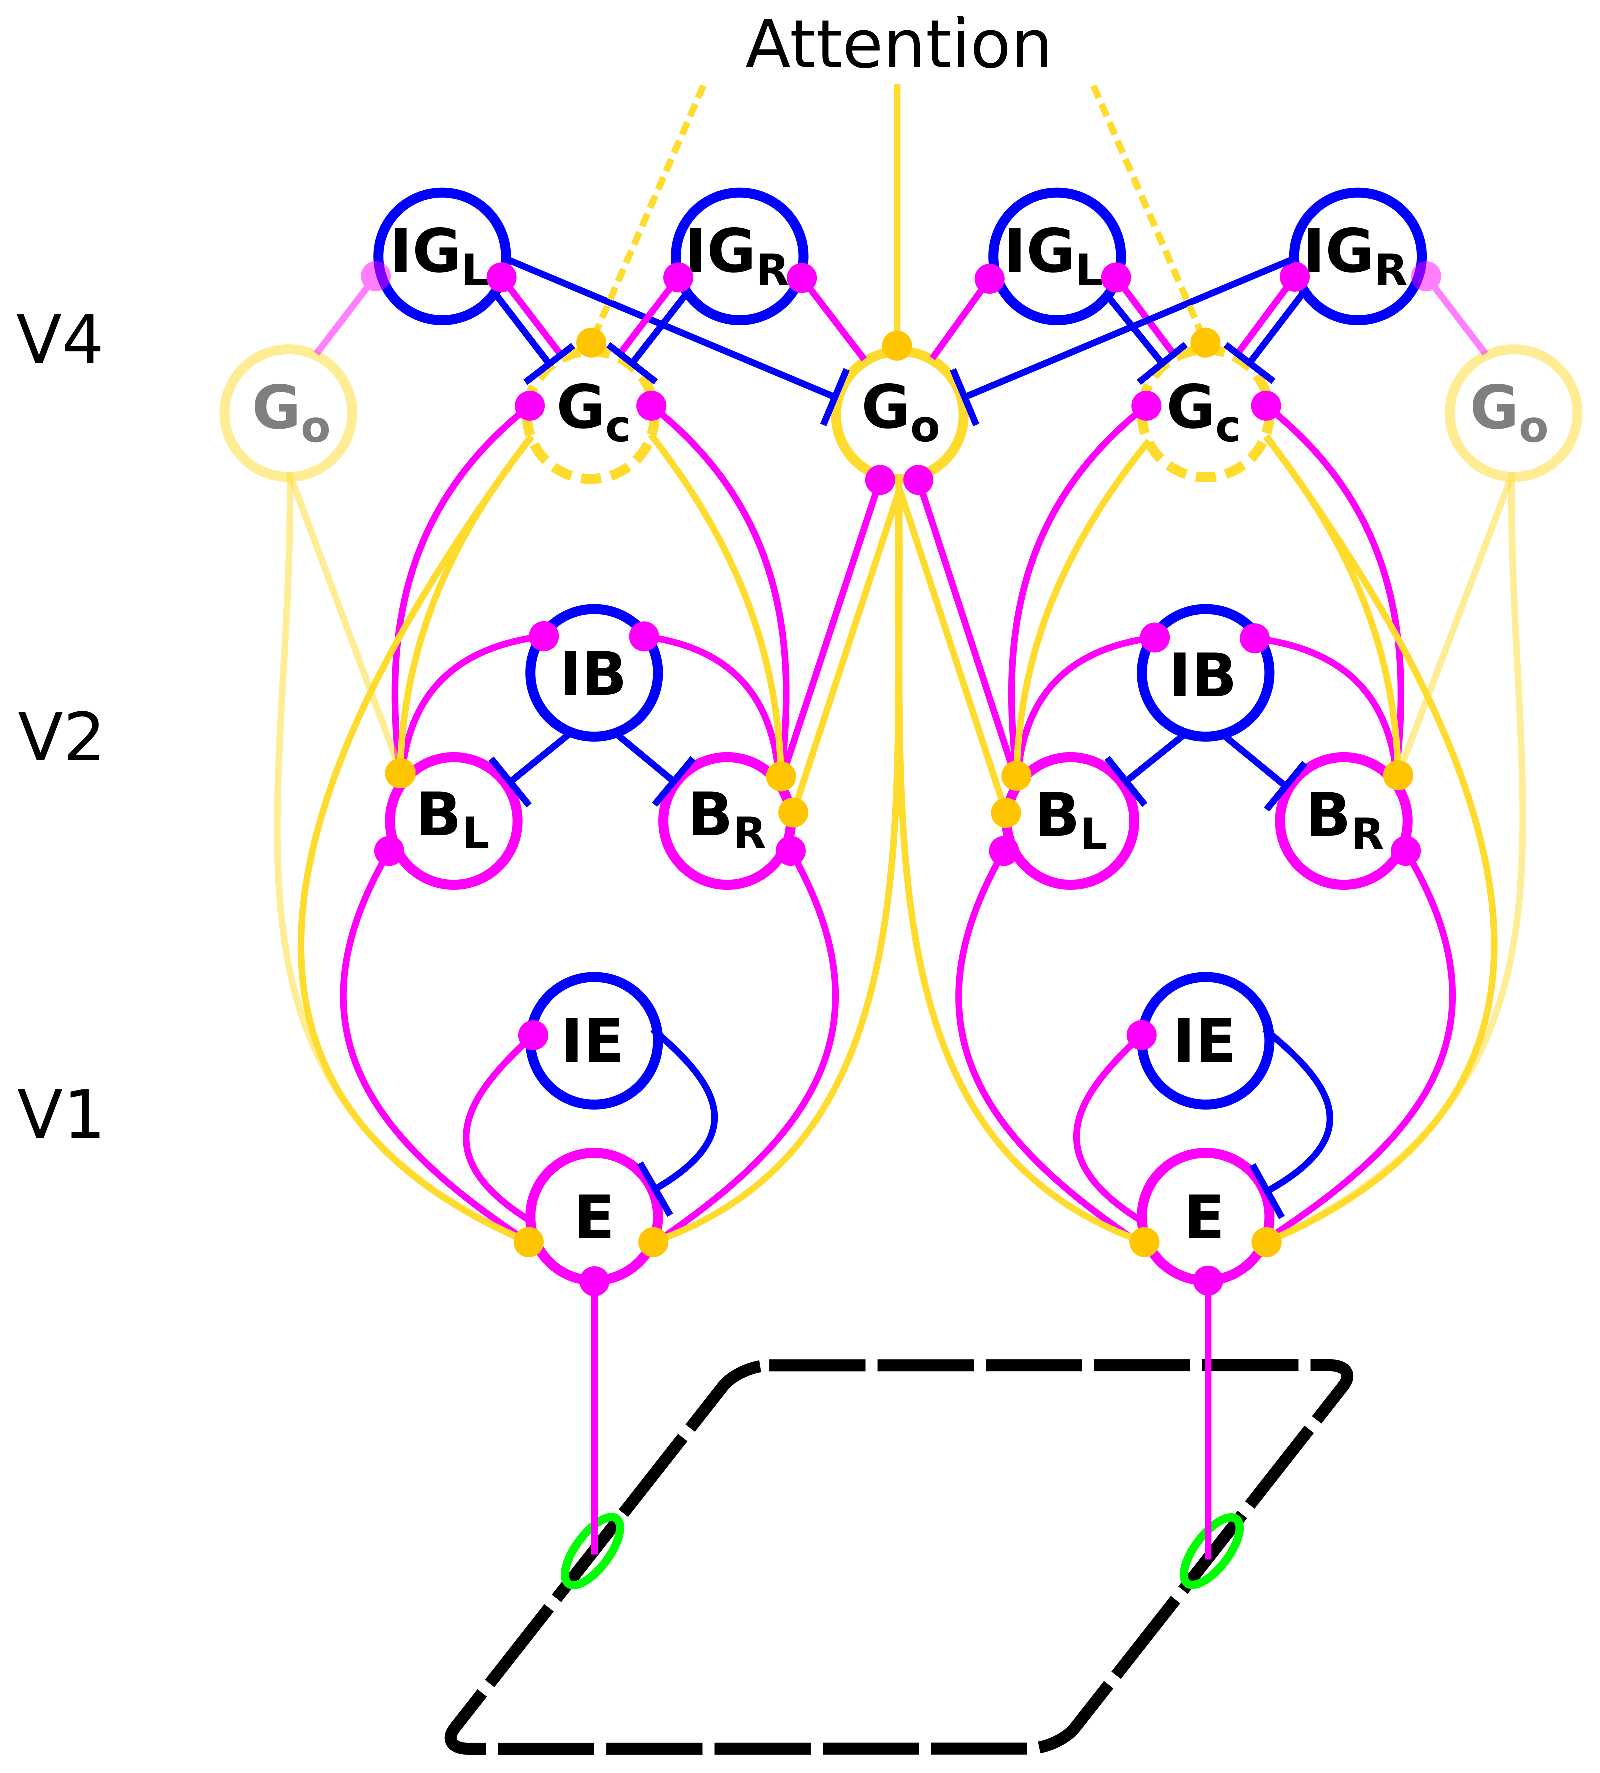
\includegraphics[width=0.5\textwidth]{Fig1.eps}
\end{center}
\caption{Structure of the model network. Each circle stands for a
  population of neurons with similar receptive fields and response
  properties.  Magenta, blue, and orange lines represent feedforward
  excitatory, lateral inhibitory, and feedback excitatory projections,
  respectively. Edges and other local features of a figure (black
  dashed parallelogram) activate edge cells (E) whose receptive
  fields are shown by green ellipses. Edge cells project to border
  ownership cells (B) that have the same preferred orientation and
  retinotopic position as the E cells they receive input
  from. However, for each location and preferred orientation there are
  two B cell populations with opposite side-of-figure preferences, in
  the example shown $B_{L}$ whose neurons respond preferentially when
  the foreground object is to the left of their receptive fields and
  $B_{R}$ whose members prefer the foreground to the right side of
  their receptive fields.\ E cells also excite other E cells with the
  same preferred orientation (connections not shown), as well as a
  class of inhibitory cells (IE) which, in turn, inhibit E cells of
  all preferred orientations at a given location. Only E cells of one
  preferred orientation are shown.  B cells have reciprocal, forward
  excitatory and feedback modulatory connections with two types of
  grouping cells, $\rm G_c$ and $\rm G_o$, which integrate global
  context information about contours and objects, respectively. E
  cells receive positive (enhancing) modulatory feedback from these same
  grouping cells. Opposing border ownership cells compete directly
  {\em via} IB cells and indirectly {\em via} grouping cells, which
  bias their activity and thus generate the response differences of
  opposing border ownership selective neurons.  G cell populations
  also directly excite inhibitory grouping cells (IG; again with the
  indices L and R), which inhibit $\rm G_c$ cells nonspecifically and
  $\rm G_o$ cells in all orientations except the preferred
  one. Top-down attention is modeled as input to the grouping cells
  and can therefore either be directed towards objects (solid lines)
  or contours (dashed lines) in the visual field (top).}
\label{Fig:anatomy}
\end{figure*}

Previous experimental studies have suggested the involvement of
multiple visual areas in contour integration and figure-ground
segregation~\citep{Poort_etal12,Chen_etal14}.  The purpose of the
present paper is to extend previous models of perceptual
organization~\citep{Craft_etal07,Mihalas_etal11b} to explain how
feedback grouping circuitry can implement the mechanisms necessary to
accomplish both contour integration and figure-ground assignment.
Most models mentioned above reproduce results restricted to a single
set of experiments (\eg contour integration or figure-ground
segregation). In contrast, our model is able to reproduce results from
at least three sets of experiments using the same set of network
parameters. Our model provides a general framework for understanding
how features can be grouped into proto-objects useful for the
perceptual organization of a visual scene. In addition, our model also
allows us to explain effects of object-based attention and the role of
feedback in parsing visual scenes, areas of research which have not
been extensively studied.

\section{Materials and methods} 
\label{sec:model}
\subsection{Model Structure}

The model consists of areas V1, V2, and V4
(Figure~\ref{Fig:anatomy}). Input comes from a
binary-valued orientation map with four orientations
($0, \pi/4, \pi/2,$ and $3\pi/4$ relative to the horizontal). The
input signal is first represented in V1 and then propagated to V2 and
V4 by feedforward connections. Area V4 provides feedback to lower
areas (see Supplementary Material for equations). Neurons in higher
areas have larger RFs and represent the image at a coarser
resolution. Linear RF sizes in area V4 are four times larger than 
in V2, which, in turn, are twice as large as those in V1.

\begin{figure*}
\begin{center}
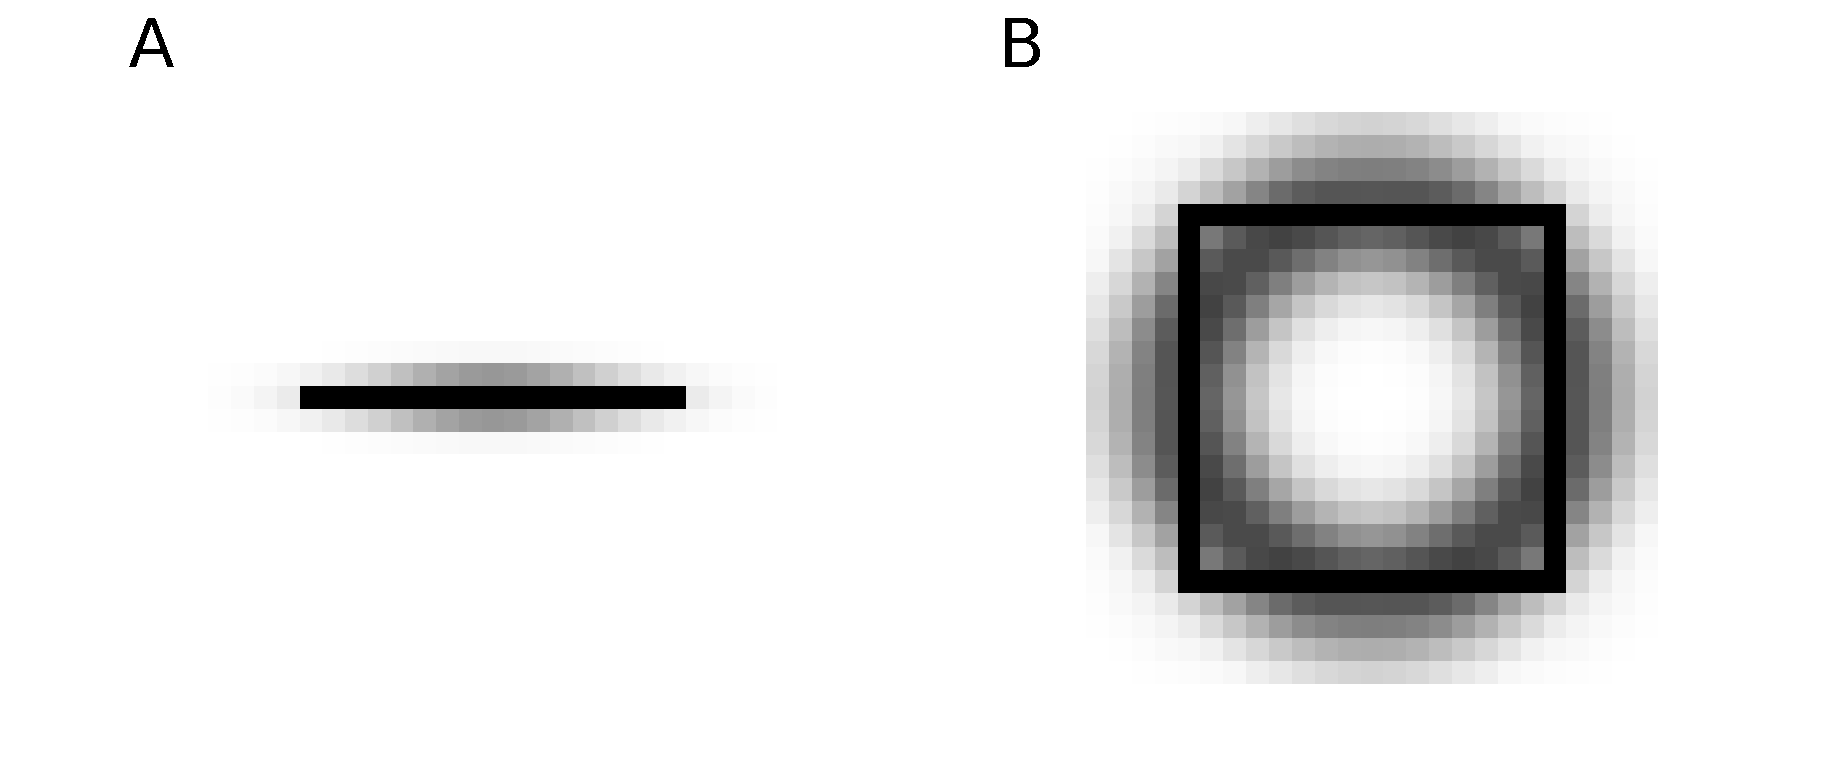
\includegraphics[width=0.75\textwidth]{Fig2.eps}
\end{center}
\caption{Spatial distribution of border ownership cell to grouping
  cell connectivity; darker pixels indicate stronger connection
  weights. A) Contour grouping neurons integrate features along
  oriented contours (horizontal line shown in black), emphasizing the
  Gestalt principle of good continuation. B) Object grouping neurons
  integrate features in a co-circular pattern (square figure shown in
  black), emphasizing the Gestalt principles of convexity and
  proximity.} 
\label{Fig:BG_projections}
\end{figure*}

To achieve contour integration, we implement 
mutual  excitatory lateral connections between V1 edge (E) cells with the same orientation
preference. These connections are similar to the local association
fields used in other models~\citep{Li98,Piech_etal13}. Background
suppression is carried out through a separate population of inhibitory
(IE) cells. The input from V1 edge cells activates border-ownership (B) cells in V2.
The B cells inherit their orientation preferences from their
presynaptic E cells and for each orientation, there are two B cell
populations with opposing side-of-figure preferences.
A combination of lateral connections within V2 and feedback connections from V4 (described
below) is used to generate border-ownership selectivity. Inhibitory
(IB) cells in V2 cause competition between B cells that have 
the same location and same orientation preference and
opposite side-of-figure preference.

In V4, two different types of grouping cells exist. Contour grouping
cells ($\rm G_c$) integrate local edge information and are selective
for oriented contours (Figure~\ref{Fig:BG_projections}A). Object
grouping cells ($\rm G_o$) are sensitive to roughly
co-circular arrangements of edges,
thus implementing Gestalt laws of good continuation, convexity of contour, and compact
shape (Figure~\ref{Fig:BG_projections}B). Competition between separate
contours and objects is carried out by a population of inhibitory (IG)
cells. Grouping ($\rm G_c$ and $\rm G_c$) cells project back 
reciprocally to those B cells from which they receive input, and also to the E
cells that project to those B cells. This feedback enhances the
activity of E cells along contours and biases the competition between
B cells to correctly assign border ownership along object
boundaries. Importantly, feedback connections are modulatory, rather
than driving, such that the feedback does not modify activities of
cells that do not receive sensory input. Biophysically, this can be achieved if the feedback projections employ
glutamatergic synapses of the NMDA type \citep{Wagatsuma_etal16a}.

To model the effect of object-based attention, we assume that areas
higher than V4 provide additional excitatory input to those grouping cells 
whose activity represents the presence of objects or contours in the visual scene, 
as shown in Figure~\ref{Fig:anatomy}. This attentional input is driving
(as opposed to modulatory) but it is relatively weak; we select its strength as 7\% of that of the
driving input to the sensory (E) cells. In one part of this study (section~\ref{sec:feedback}), we 
model the effect of a lesion in V4 that removes the feedback completely by setting the
weight of feedback connections from V4 to lower areas to zero.

Our approach is an extension of the proto-object-based model of
perceptual organization proposed by \cite{Mihalas_etal11b}. Different
from their approach, we include a new population of contour grouping
neurons (the $G_c$ cells) to explain recent results on cortico-cortical interactions
during contour integration~\citep{Chen_etal14}. As a result, top-down
attention in our model can either be directed to 
contours or to objects. Our model is also able to reproduce
the time course of neural responses in different visual areas, while
the \cite{Mihalas_etal11b} model only explains mean neural
activities. In order to create more complex input stimuli, we also
increased the number of model orientations from two to four. As a
simplification to their model, we only include one scale of grouping
neurons since we focus on mechanisms that do not require multiple
scales.

\subsection{Model Implementation}
\label{sec:implementation}
Model neuronal populations (usually referred to as ``neurons'' in the
following) are represented by their mean activity (rate coding).  The
activity is determined by a set of coupled, first-order nonlinear
ordinary differential equations which was solved in MATLAB (MathWorks,
Natick MA) using standard numerical integration methods.  The mean
firing rate is necessarily positive, therefore units are simple
zero-threshold, linear neurons which receive excitatory and inhibitory
current inputs with their dynamics described by,
\begin{equation}
\label{eq:1}
\tau f'(t) = -f + \left[ \sum W \right]_{+}
\end{equation}
where $f$ represents the neuron's activity level and $\tau$ its time
constant, chosen as $\tau$ = $10^{-2}$ s for all neurons. The sum is
over all $W$ which are the neuron's inputs,
$f'$ is the first derivative of $f$ with respect to
time, and $[\,]_{+}$ means half-wave rectification.

All simulations were performed on a 300-core CPU cluster running Rocks
6.2 (Sidewinder), a Linux distribution intended for high-performance
computing.  A total of 100 simulations were performed for each
experimental condition, and our results are based on the mean neural
activities averaged over these simulations with different randomly
selected stimulus noise patterns, see sections~\ref{sec:contour_exp}
and~\ref{sec:FGO}.

To constrain our model parameters, we used three sets of
neurophysiological data. The first comes from recent contour grouping
results~\citep{Chen_etal14}, and our model was able to largely
reproduce the magnitude and time course of contour integration at both
the V1 and V4 levels. The second comes from studies of border-ownership coding
\citep{Zhou_etal00} and we show that our model not only explains the
emergence of border ownership selectivity but also its approximate
time course as reported in that study. The third set of experimental data
constraining our model is from the study by \cite{Qiu_etal07} of the
interaction between border-ownership selectivity and selective
attention. In order to fit the model
parameters, we started from the parameters given by
\cite{Mihalas_etal11b}, and modified them to fit the larger body of
experimental results to include contour integration, border-ownership
selectivity, and attentional selection.

\subsection{Contour integration experiments} 
\label{sec:contour_exp}
For the contour integration experiments reported by
\cite{Chen_etal14}, awake behaving monkeys were trained to perform a
two-alternative forced-choice task using two simultaneously presented
patterns, one containing a contour embedded in noise and one that was
noise only (see Figure~\ref{Fig:Contour_Results} for examples).  The
patterns were composed of $0.25^{\circ}$ by $0.05^{\circ}$ bars
distributed in $0.5^{\circ}$ by $0.5^{\circ}$ grids.  The diameter of
the patterns was $4.5^{\circ}$, and the number of bars in the embedded
contour was randomly set to 1, 3, 5, or 7 bars within a block of
trials in order to control the saliency of the contour.  To obtain a
reward, the monkey had to saccade to the pattern that contained the
contour. When the number of bars was set to 1, both presented
stimuli were noise patterns, and the monkey was rewarded 
randomly with a probability of 50\%.  While the animals were performing the task,
simultaneous single- or multi-unit recordings were made in area V1 and
V4 neurons with overlapping receptive fields.

\begin{figure*}[t!]
\begin{center}
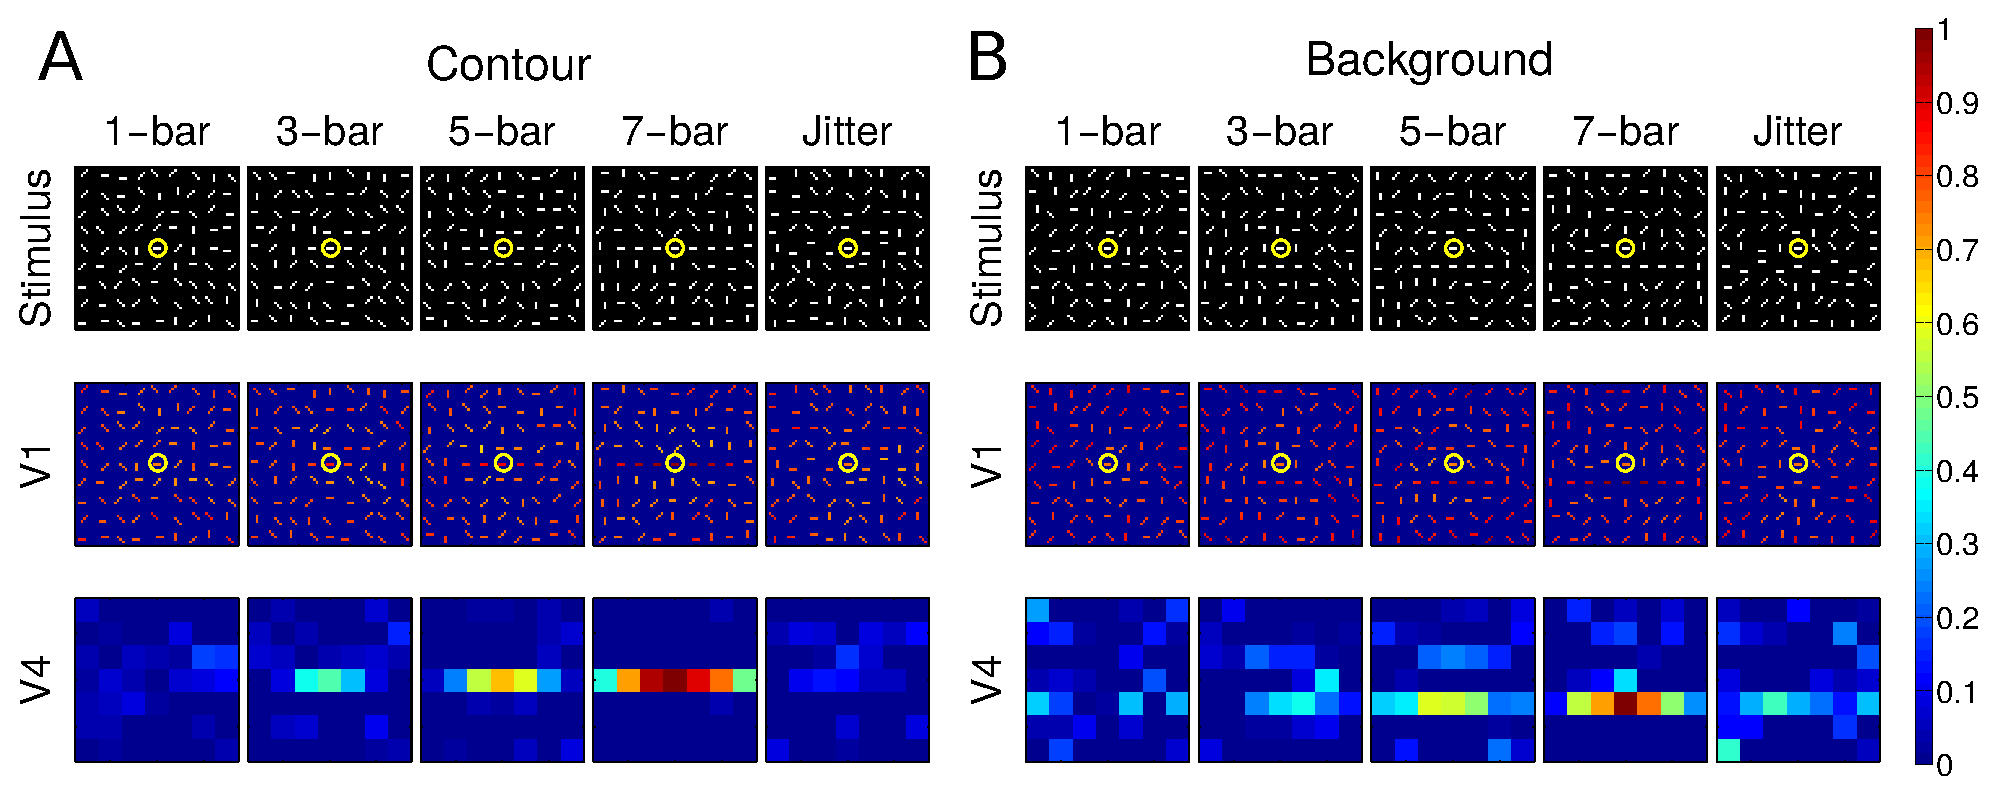
\includegraphics[width=0.75\textwidth]{Fig3.eps}
\end{center}
\caption{Normalized V1 $E$ cell and V4 $G_c$ cell population responses
 to contours of varying lengths in either the contour (A) or the background (B)
condition. In (A), the ``recorded'' neuron is on the contour; in
(B), it is offset from the contour. The top row shows stimuli, the
second and third rows show activity in model areas 
V1 and V4, respectively. Yellow circles mark the RFs of the V1 neurons whose activity is shown in Figure~\ref{Fig:Neural_responses}.
Activity from model area V2 is not shown because a single contour does
not produce clear border ownership selectivity, and the activity in V2
is essentially the same as that in V1, but with reduced spatial
resolution due to the lower number of neurons.  
Columns in each condition show, from left to right, increasing
contour length, with the right-most column showing a jittered stimulus
configuration (see text). Neural activity is color coded
and normalized to the 7-bar stimulus in both contour and background conditions,
with warmer colors representing higher activity (see color bar at right).
To avoid unbalanced inputs near the boundaries of the visual field we use periodic boundary
conditions. We crop this and all other maps of population activity by one pixel on each
side to remove artifacts related to using periodic boundary conditions.
}
\label{Fig:Contour_Results}
\end{figure*}

We modeled these experiments by creating visual stimuli contained in a
$4.5^{\circ}$ by $4.5^{\circ}$ area. We ``recorded'' from the V1 receptive
field that was at the center of the stimulus (marked by the yellow
circles in Figure~\ref{Fig:Contour_Results}), as well as from the
corresponding V4 neuron. Input from this
area was projected onto a V1 layer of $64 \times 64$
neurons, each with a receptive field size of $\sim0.7^{\circ}$ so the
receptive fields overlapped ten-fold at each location in the visual
field.  We divided the input field into a $9 \times 9$ grid (each grid
point at the center of a $0.5^{\circ}$ by $0.5^{\circ}$ area) and we
placed at each grid location a stimulus bar 
consisting of three adjacent pixels, corresponding to a size
$\sim0.21^{\circ}$ by $\sim0.07^{\circ}$. 
Each stimulus bar had one of four orientations, $0, \pi/4, \pi/2,$ or
$3\pi/4$.  As in the \cite{Chen_etal14} experiment, contours consisted of 1, 3, 5, or 7 adjacent
stimulus bars. We positioned the contour either 
at the center of the visual field so that the center element of the contour was in the RF of the
``recorded'' cell (Contour condition,
Fig.~\ref{Fig:Contour_Results}A), or offset from the center of the
visual field, such that the ``recorded'' neuron was {\em next} to the
contour (Background condition, Fig.~\ref{Fig:Contour_Results}B).
We changed the length of the contour by adding bars
to both ends of the contour. Due to their size, V4 receptive fields basically enclosed the entire
contour. For more details on the stimulus configuration, see Section~\ref{sec:contour}.

\subsection{Figure-ground segregation experiments} 
\label{sec:FGO}
For the figure-ground segregation experiments~\citep{Zhou_etal00,
  Qiu_etal07, Zhang_vonderHeydt10}, awake, behaving monkeys were
trained on a fixation task.  Receptive fields of each recorded neuron
in areas V1 and V2 were first mapped to determine the optimal stimulus
properties for that neuron. Afterwards, in some experiments, a square
shape was presented on a uniform gray background with one edge of the
square centered on the receptive field of the neuron at the neuron's
preferred orientation.  In other experiments (results shown in
Figures~\ref{Fig:Overlap_Square_exp_model}
and~\ref{Fig:Overlap_Square}) the stimulus consisted of two partially
overlapping squares, and again the receptive field of the recorded
neuron was centered at its preferred orientation on one edge of one of
the squares.  The size of the square varied between experiments but it
was always chosen such that the closest corner was far away from the
classical receptive field of the recorded neuron. The square was
presented in two positions between which it was ``flipped'' along the
long axis of the neuron's receptive field. For instance, if the
preferred orientation was vertical, the square was presented either to
the left or the right of the cell's receptive field (we used this
example in the choice of the indices in Figure~\ref{Fig:anatomy}).
The difference in the firing rate of the neuron for when the square
appears on one side versus the other side is defined
as the border-ownership signal. Importantly, in all stimulus conditions, local 
%bh are you sure you want to use the word "contents"? do you mean "context" instead in contrasting local vs. global?
contents 
%
within the receptive field of the neuron remained the same between
these two conditions; only global context  
changed, so the neuron had to integrate information from
outside its classical receptive field.

We modeled these experiments by creating visual stimuli that were
projected onto the V1 layer. The input to the simulation was either a
single square of a size that maximally activated $\rm G_o$ grouping
cells of the size chosen in our model, or two partially overlapping
squares, as shown in Figure~\ref{Fig:Overlap_Square}, with each of
these squares having the same optimal size. In other models
\citep{Craft_etal07,Mihalas_etal11b,Russell_etal14}, grouping cells of
many scales are present, covering the range of possible objects in the
input. We calculated border-ownership selectivity at the V2 level
using the vector modulation index defined in section~\ref{sec:vmi}.
In order to create noisy versions of the single square image
(Figure~\ref{Fig:Square_Noise}), we followed a similar approach as in
the contour integration experiments, section~\ref{sec:contour_exp}.
We again divided the visual field into a $9 \times 9$ grid and we
positioned horizontal and vertical bars at specific grid points to
generate a square. We then placed a stimulus bar at all other grid
points, with their orientations randomly chosen from four
possibilities, $0, \pi/4, \pi/2,$ and $3\pi/4$.

\begin{figure*}
\begin{center}
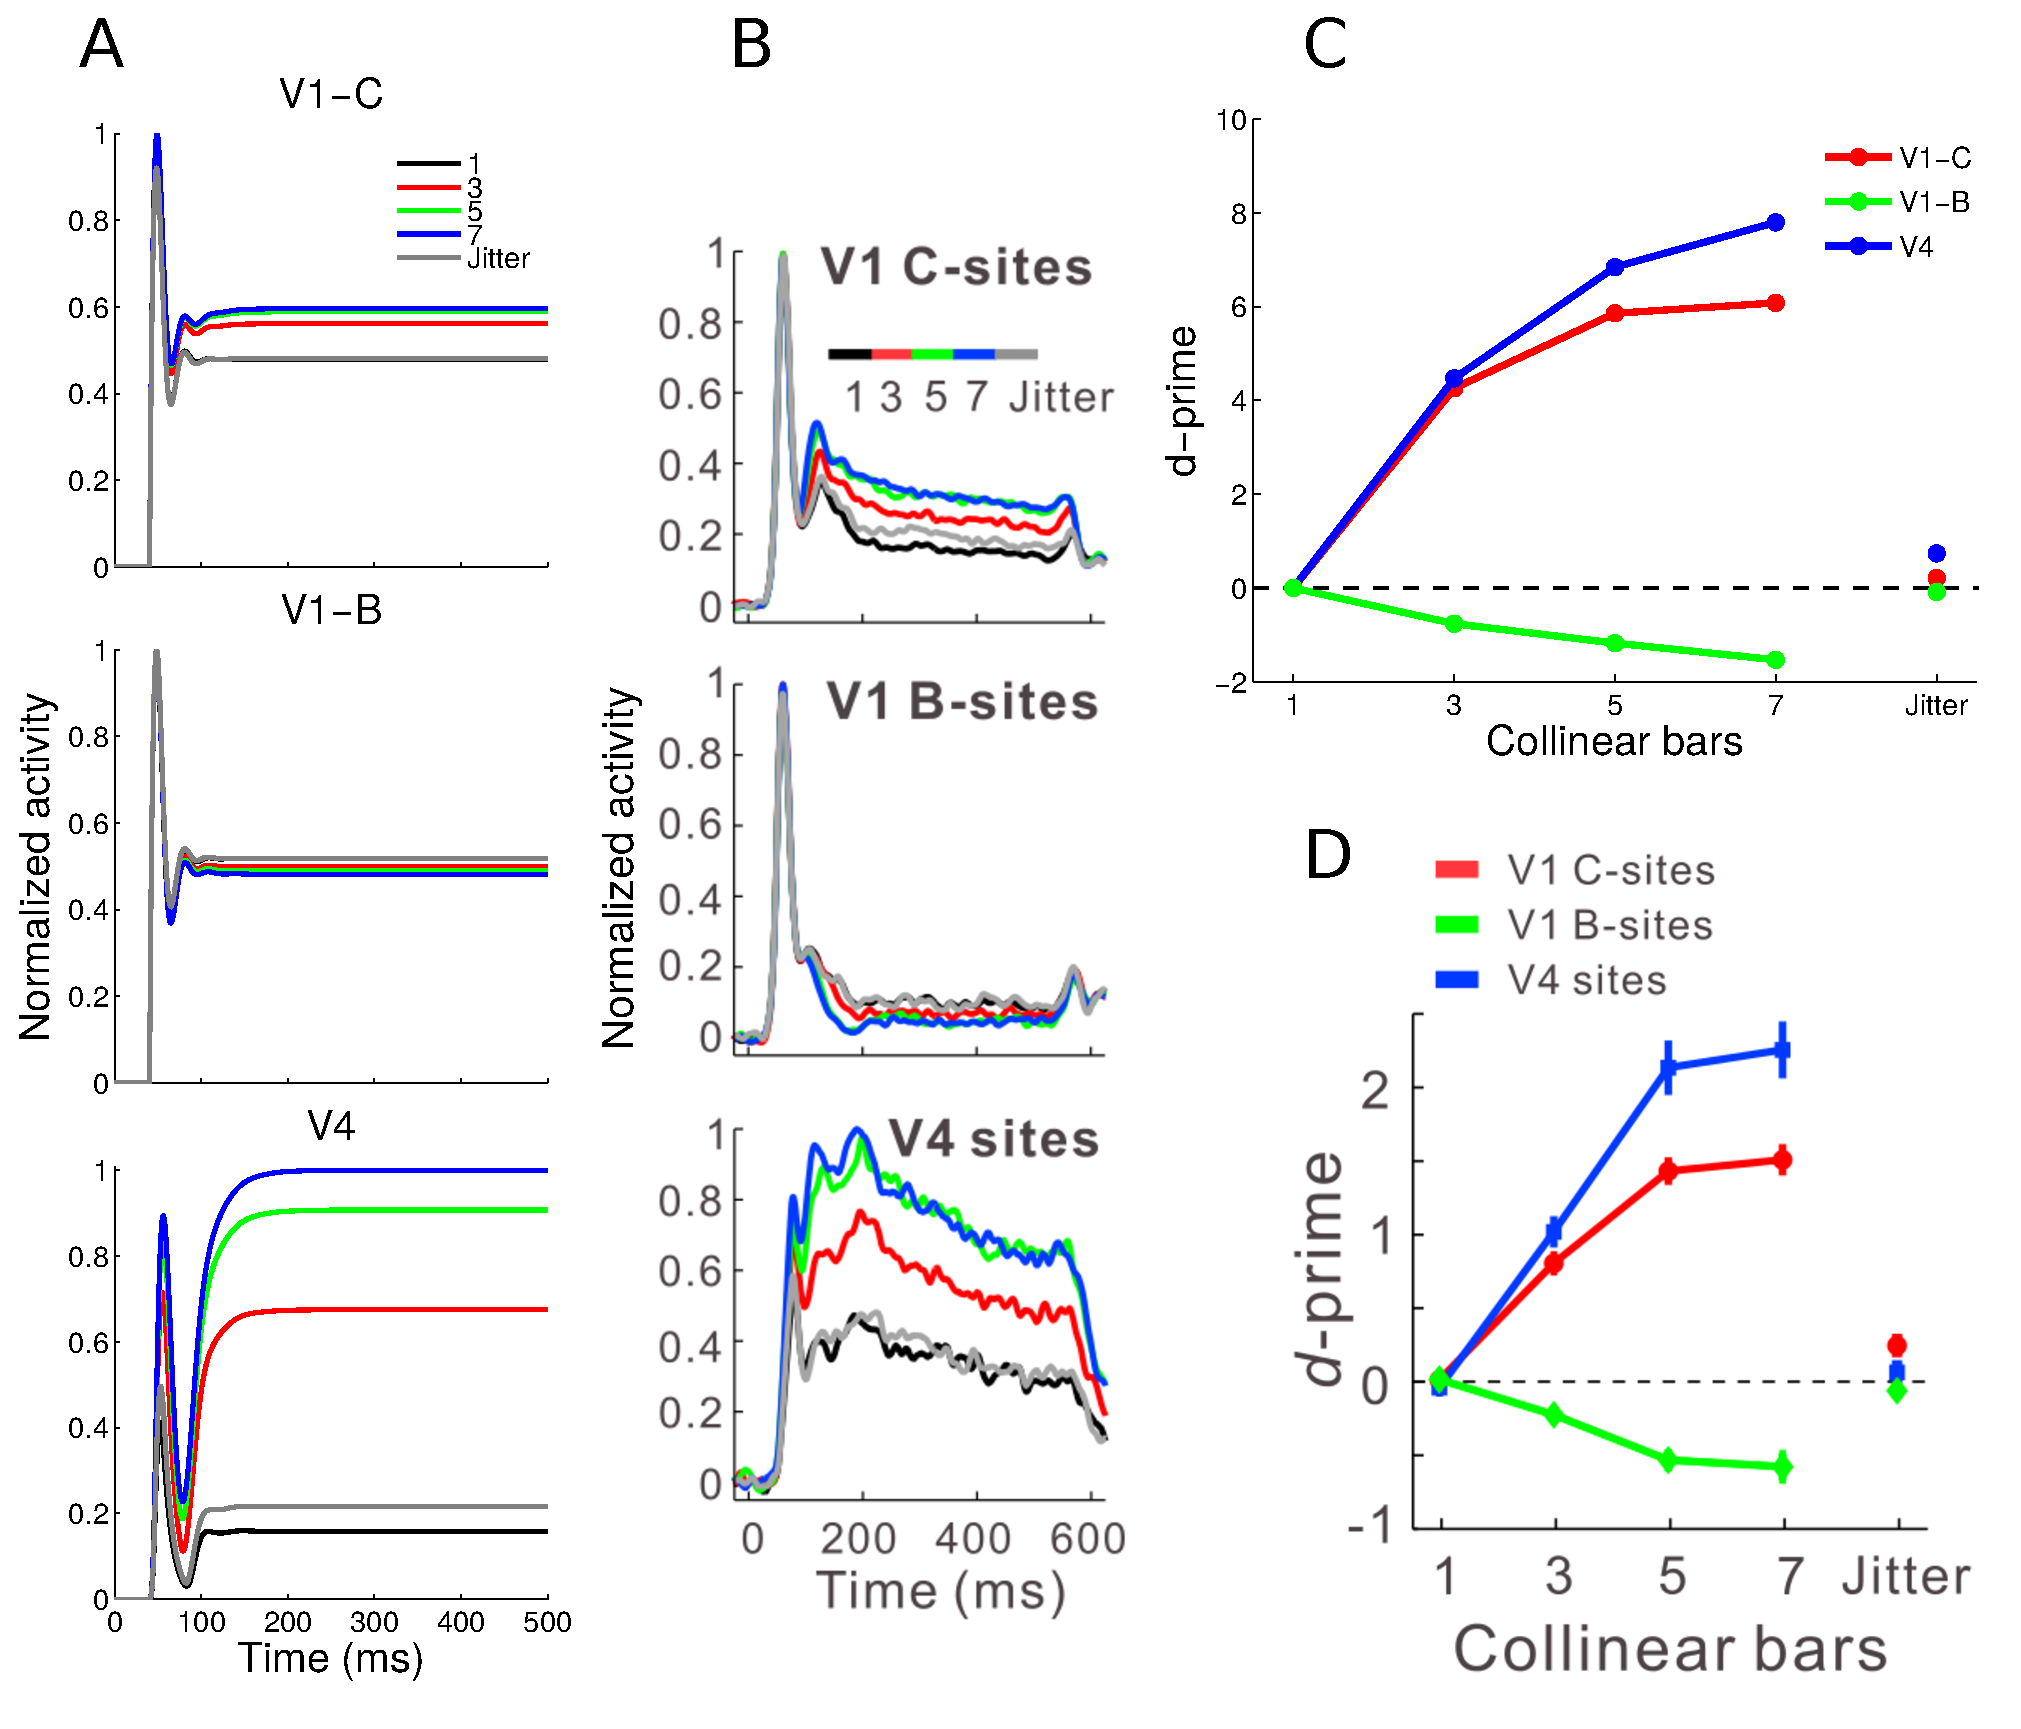
\includegraphics[width=0.75\textwidth]{Fig4.eps}
\end{center}
\caption{Normalized V1 $E$ cell (contour and background sites) and V4
  $G_c$ cell neuronal activity and contour-response $d'$ to contours of
  varying lengths. (A) V1 contour (top) and background (middle) sites
  and V4 sites (bottom) showed facilitation followed by saturation
  with increasing contour length (see legend). V1 background sites
  showed greater suppression with longer contours. The jitter
  condition involved a 7-bar pattern where each bar was laterally
  offset to disrupt collinearity. (B) Corresponding experimental
  results showing normalized and averaged PSTHs from
  the~\cite{Chen_etal14} study. 
  (C) Contour-response $d'$ was higher for the V4
  sites compared to the V1 contour sites, and was facilitated by
  increasing contour length. V1 background sites had increasingly
  negative $d'$ with longer contours, indicating background
  suppression. The jitter condition reduced the absolute value of the
  $d'$ values to close to zero, making it similar to the baseline
  noise condition. (D) Corresponding experimental observations,
  showing the mean contour-response $d'$ from the~\cite{Chen_etal14}
  study. Panels B and D are modified from Figure~2 of~\cite{Chen_etal14}.
  All model results (Panels~A and~C) are averages for a single neuron over 100 simulations.}
\label{Fig:Neural_responses}
\end{figure*}

\subsection{Quantitative assessment of border ownership selectivity:  Vector modulation index}
\label{sec:vmi}
While the border ownership signal discussed in the previous
section (the difference in firing rates between presentations of a figure
on the two sides of a a neuron's RF) is useful to
characterize border-ownership selectivity for that particular neuron,
description of population behavior requires a more general measure. We
use the vector modulation index, introduced by \cite{Craft_etal07} and defined
by the expression 
\begin{equation}
\label{eq:2}
\vv{\mathbf{v}}(x,y) = m_{\hat{\imath}}(x,y)\hat{\imath} + m_{\hat{\jmath}}(x,y)\hat{\jmath}
\end{equation}
where $\hat{\imath}$ and $\hat{\jmath}$ are unit vectors along the horizontal and vertical image
axis, respectively, and the components $m_{\hat{\imath}}(x,y)$ and $m_{\hat{\jmath}}(x,y)$ are the usual modulation indices along their respective axes, defined as
\begin{equation}
\label{eq:3}
\begin{split}
	m_{\hat{\imath}}(x,y) = \frac{\sum_{\theta}
        B_{\theta}(x,y)\cos\theta}{\sum_{\theta}
                \left|B_{\theta}(x,y)\cos\theta\right|} \\
	m_{\hat{\jmath}}(x,y) = \frac{\sum_{\theta}
        B_{\theta}(x,y)\sin\theta}{\sum_{\theta}
                \left|B_{\theta}(x,y)\sin\theta\right|}
\end{split}
\end{equation}
Here, $B_{\theta}(x,y)$ is the border ownership signal (difference between
the activities of the two opposing B neurons) at the preferred
orientation $\theta$ at position $(x,y)$, and $\theta$ runs over all
angles taken into account in the model 
(four directed orientations in our case, namely $0, \pi/4, \pi/2,$
and $3\pi/4$, each with both side-of-figure preferences). 
Vertical bars in the sums in the denominators indicate absolute values.

Both components in Eq.~\ref{eq:3} are limited to values between +1 and
-1. For the x-component, for instance, a positive value of
$m_{\hat{\imath}}(x,y)$ signifies that the figure is to the right of
position (x,y) and a negative value signifies that the figure is to
the left. Its absolute value indicates the ``strength'' of the
border-ownership signal, with zero being equivalent to ambivalence
between left and right. Corresponding comments apply to the
y-component, $m_{\hat{\jmath}}(x,y)$, regarding the figure's position
upward or downward of (x,y). The direction of the vectorial modulation
index $\vv{\mathbf{v}}(x,y)$ 
defined in Eq.~\ref{eq:2} indicates the position
of the foreground figure in the two-dimensional image plane relative
to the point (x,y). For instance, positive values in both components
[$m_{\hat{\imath}}(x,y) > 0$, $m_{\hat{\jmath}}(x,y) > 0$] indicate
that the figure is located upwards and to the right of (x,y).

\section{Results}
\label{sec:results}
\subsection{Contour enhancement in V1 and V4}
\label{sec:contour}
We examined contour-related responses in our model using visual
stimuli composed of collinear bars among randomly oriented bars
(Figure~\ref{Fig:Contour_Results}), closely matching the stimuli used
in the physiological experiments by \cite{Chen_etal14}. The number of
collinear bars constituting an embedded contour was set to either 1,
3, 5, or 7 bars, determining the length of the embedded contour, which
also controlled its saliency.  When the number of collinear bars was
one, the stimulus was identical to a noise pattern. We compared the
activity of model neurons whose RFs are centered on the contours or in
the noise background (but close to contours) with that obtained in the
analogous positions during neurophysiological recordings.

V1 responses were split into those of neurons on contour sites
(C-sites) and background sites (B-sites). For contour sites
(Figure~\ref{Fig:Contour_Results}A), the embedded contour was centered
on the RF of a neuron with a preferred orientation matching that of
the contour. For background sites, the contour was laterally placed
0.5$^{\circ}$ away from the RF center of the recorded neuron, and a
background bar was placed in the RF
(Figure~\ref{Fig:Contour_Results}B), with the contour orientation
again matching the preferred orientation of the recorded neuron.
Both V1 and V4 neurons along the contour showed increased activity with contour length. Neurons on the background showed increased suppression with contour length.
Correspondingly, we show in Figure~\ref{Fig:Neural_responses} the
responses of neurons whose preferred orientations align with the
contours (yellow circles in Figure~\ref{Fig:Contour_Results}).

Except for an input delay of 40ms corresponding to the duration of
visual processing from the retina to V1, we did not 
add any time delays in the feedforward or feedback connections of
our model, as we were not attempting to reproduce 
any specific latency effects.
Nevertheless, our model generally reproduced the dynamics of neural
responses to contours in both V1 and V4 observed in the
\cite{Chen_etal14} experiment (Figure~\ref{Fig:Neural_responses}A).
The most salient feature of the neuronal responses is that the levels
of sustained activity differ based on the number of bars in the
embedded contour. This is observed both for contour sites and for
background sites but, importantly, this effect went in opposite
directions for these two cases.  As the number of collinear bars
increased from one to seven, V1 contour sites centered on the contour
showed increased activity, with response saturation after five
bars. In contrast, V1 background sites that were offset from the
embedded contour showed a decrease in activity with increasing number
of bars in the background (response suppression). Similar to V1
contour sites, V4 sites showed saturating responses with increasing
contour lengths (Figure~\ref{Fig:Neural_responses}A, bottom).  These
results were qualitatively similar to those obtained in
the~\cite{Chen_etal14} experiments which are reproduced in
Figure~\ref{Fig:Neural_responses}B (their Figure~2A).

The model data also showed strong onset transients in both (contour
and background) V1 populations (Figure~\ref{Fig:Neural_responses}A,
top and center), again in good agreement with experimental results
(Figure~\ref{Fig:Neural_responses}B, top and center). Transients in V4
neurons were weaker, in both model and experimental data, and nearly
absent in the experimental data (though not the model) for longer
contours (Figure~\ref{Fig:Neural_responses}B, bottom).
The transient peak observed in the model results
is due to a sharp suppression of the activity level for a short
($<50$ms) period which is not observed in the empirical data. We
believe that this suppression is due to the  strong inhibition at the
V4 level between G and IG cells, without equivalent
excitation between different G cells.

\begin{figure*}
\begin{center}
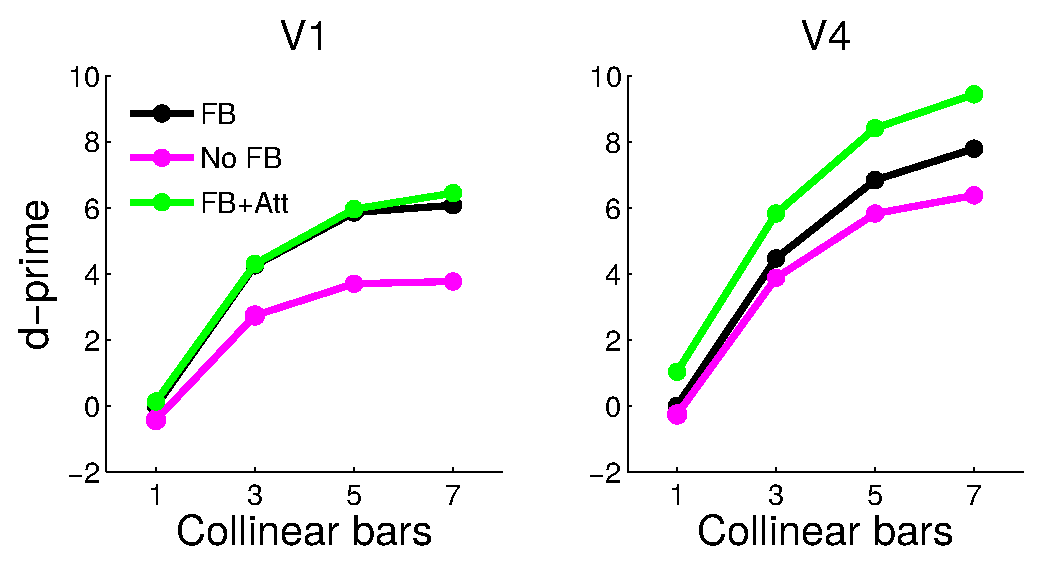
\includegraphics[width=0.75\textwidth]{Fig5.eps}
\end{center}
\caption{Contour-response $d'$ in V1 $E$ cells (A) and V4 $G_c$ cells (B) for the model with (green) and without attention (black), and for the model with feedback removed 
(magenta). Attention strongly increased
  contour-response $d'$ in V4 (B), while the lack of feedback strongly
  decreased contour-response $d'$ in V1 (A).}
\label{Fig:FB_att}
\end{figure*}

Following \cite{Chen_etal14}, 
we quantitatively analyzed the contour responses using the d-prime
$(d')$ metric from signal detection theory~\citep{Green_Swets66}, which
quantifies the difference in distributions of mean neuronal firing
rates between a contour pattern and the noise pattern integrated over
the whole interval shown in Figure~\ref{Fig:Neural_responses}A,B, \ie
0-500 ms.  Neuronal responses to the 1-bar pattern (the noise pattern)
were the baseline for examining contour-related responses in V1 and
V4, this pattern therefore had a contour-response $d'$ of zero. The
contour-response $d'$ increased with contour length for both the V1
contour and V4 sites, and $d'$ decreased with contour length for the V1
background sites, Figure~\ref{Fig:Neural_responses}C.

The agreement between model (Figure~\ref{Fig:Neural_responses}C) and
experimental results (Figure~\ref{Fig:Neural_responses}D) is striking.
One difference we note is that the absolute values of all model $d'$
substantially exceed the corresponding experimental values. 
This is to be expected since no noise was included in the model 
(other than the random orientation of input
stimulus bars which is also present in the experimental approach)
while there are surely multiple sources of noise in the biological
system. We have not thoroughly investigated this question but it is
highly likely that addition of noise to the model will decrease the $d'$
values.

At first sight, it seems possible that 
V4 neurons respond with a higher firing rate to longer contours than
to shorter ones simply as a consequence of 
the large size of RFs in V4. 
In this view, the enhanced responses in V4 with increasing contour
length is due to the spatial summation of many bars
within the RF at the optimal orientation,
independent of their precise location in the RF. 
To  investigate this possiblity,
~\cite{Chen_etal14} introduced a ``jitter'' condition to the 7-bar
contour, where alternating collinear bars were laterally offset 
by a small amount (much less than the receptive field size)
in order to disrupt the collinearity of the original contour. They
showed that jittering disrupted the 
contour integration process and reduced the neural responses in V1
and V4 close to baseline levels (Figure~\ref{Fig:Neural_responses}B,
gray lines). We found the same result in our model,
Figure~\ref{Fig:Neural_responses}A, gray lines.  Furthermore, in the
jitter condition, contour-response $d'$ approached baseline for the
V1 and V4 sites, as shown in the rightmost points for
Figure~\ref{Fig:Neural_responses}D for experimental data and
Figure~\ref{Fig:Neural_responses}C for model results. In both cases,
no substantial difference between the jitter condition and the
baseline noise condition was observed.

We also investigated the orientation and position dependence of
contour-related responses in V1 and V4, and found close agreement of
our model results with experimental data~\citep{Chen_etal14}. Due
to space constraints, these results are presented in the Supplementary
Material. The results for V4 are presented in Supplementary Figure~\ref{Fig:V4_total} and the results for V1 are presented in Supplementary Figure~\ref{Fig:V1_total}.

\subsection{The role of feedback and attention in contour grouping}   
\label{sec:feedback}
While different forms of attention exist that can be flexibly used for
different tasks, we choose here to focus only on the mechanisms of
object-based attention
\citep{Egly_etal94,Scholl01,Kimchi_etal07,Ho_Yeh09}.  We postulate
that attention to objects acts at the level of grouping neurons, in
agreement with the \cite{Mihalas_etal11b} model.  As shown in that
study, modulation of the activity of grouping cells bypasses the need
for attentional control circuitry to have access to detailed object
features.  Instead, grouping neurons are used as ``handles'' of the
associated objects and it is in their interaction with feature-coding
neurons that features are assigned to objects. One of the consequences
of this mechanism is that the spatial resolution of attentional
selection is coarser than visual resolution since the smallest
``unit'' of spatial attentional deployment is the size of the
receptive (and projective) field of grouping cells, which is
considerably larger than the receptive fields of feature-coding
neurons at the same eccentricity. Behavioral results show strong
evidence in favor of this coarse attentional
resolution~\citep{Intriligator_Cavanagh01}.

In our model, attention can be directed to objects, including
contours. For the contour integration experiments, this is implemented
as a top-down input to all contour grouping neurons 
at the attended location, but, importantly, 
%bh reads a little awkwardly, how about adding this?
there was
%
no direct input to the feature-coding edge (E) cells.
As we have seen before (Figure~\ref{Fig:Neural_responses}), $d'$ in V1
and V4 populations increases with the number of collinear bars, even
in the absence of attention.  In addition, we now show that attention
increases the contour-response $d'$ for both V1 and V4 neurons, with
the additive effect being much larger in V4 than in V1
(Figure~\ref{Fig:FB_att}). For the 7-bar contours, attention increases
the contour-response $d'$ in V1 from 6.08 to 6.66 and in V4 from 7.80
to 11.59. This is consistent with findings that attention has a much
larger effect on higher-level neurons compared to early sensory
neurons~\citep[review:][]{Treue01}.

One of the advantages of computational modeling is that it allows the
study of scenarios that are difficult to implement empirically.
One question that is difficult to answer experimentally is how removal of
feedback from V4 to lower visual areas
would change neuronal responses in V1 and V4, structures that
are known to be connected bidirectionally
\citep{Zeki78b,Ungerleider_etal07}.
While it is possible to study the influence of feedback on V2 (and
other areas) by cooling \citep{Hupe_etal98} or pharmacological
inactivation~\citep{Jansen-Amorim_etal12} 
of area V4, such manipulations only
allow limited control of the effect on multiple brain structures. In
contrast, a computational model allows the study of interactions
between different areas with perfect control. In the model, 
we can eliminate all feedback from area V4 simply by ``lesioning'' the
connections from the grouping neurons to the V2 and V1 neurons
(setting their strength to zero), thus turning the model into a
feedforward network.  We found that this has the opposite effect of
applying attention on the $d'$ metric: the decrease in contour
response $d'$ was much larger in V1 compared to V4. Removing feedback
reduced the 7-bar contour-response $d'$ in V1 from 6.08 to 3.77, and
in V4 from 7.80 to 6.38 (Fig.~\ref{Fig:FB_att}). We note that the
contour-response $d'$ in V1 is above zero even without feedback from
grouping neurons because of the contribution of local excitatory
connections to contour integration.  This asymmetric effect in contour
response $d'$ in the two areas (V1 and V4) may point to the different
roles of feedforward and feedback processing in early vision. We are
not aware of any experimental manipulations that completely remove
feedback from area V4 without changing the circuitry in other ways, so
our results are a prediction awaiting experimental falsification.

\begin{figure*}[t]
\begin{center}
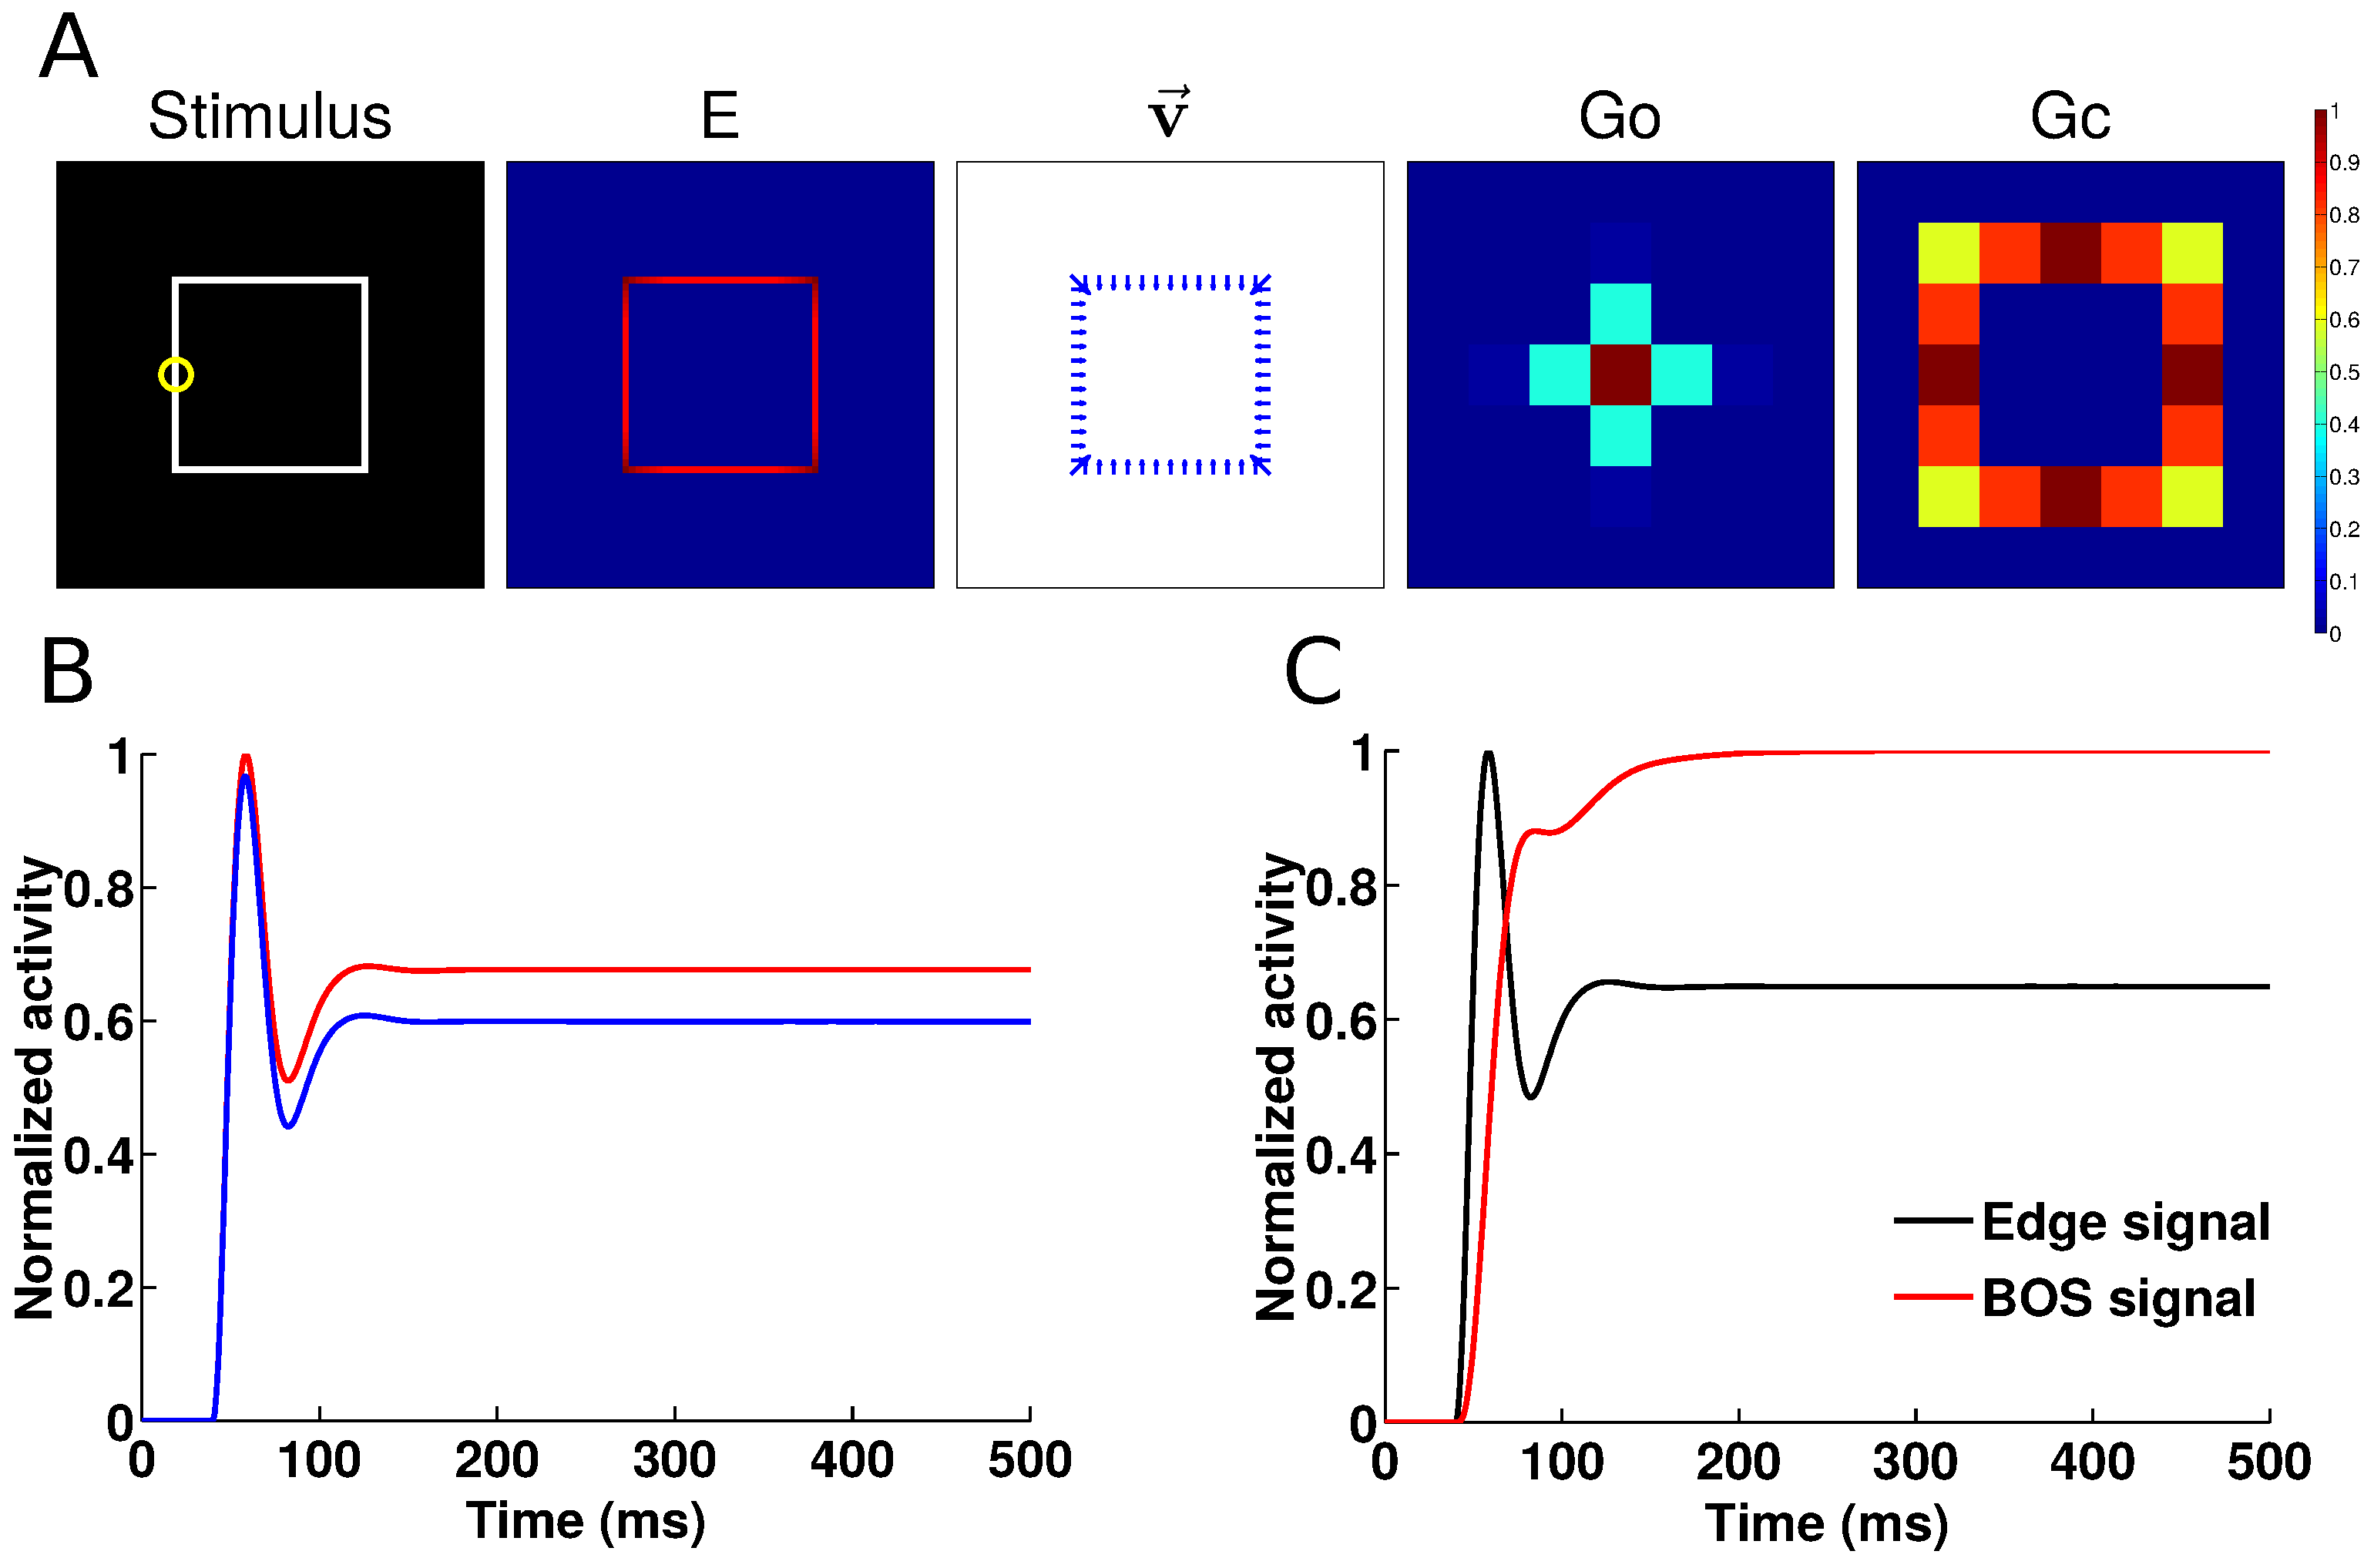
\includegraphics[width=0.75\textwidth]{Fig6.eps}
\end{center}
\caption{Figure-ground segregation of a square object as in
  the~\citet{Zhou_etal00} experiments. (A) Shown left to right are the
  input 
  stimulus, the edge cell activity (E), the border ownership
  assignment along edges (shown as the vector modulation index 
  $\protect\vv{\mathbf{v}}$,
  section~\ref{sec:vmi}),
 the object grouping 
  neuron activity 
$(G_o)$
 and the contour grouping activity
$(G_c)$.
 Activities are normalized within each map, and warmer colors
  indicate higher activity (see color bar at right). (B) Time course
  of normalized border-ownership cell activity for the preferred
  side-of-figure (red) and non-preferred side-of-figure (blue) for the
  receptive field marked by the yellow circle in panel A. Here, the
  preferred side-of-figure is to the right. (C) Timing of the
  normalized border-ownership signal (red) and the edge signal
  (black). The BOS signal is defined as the difference in activities
  of the two opposing pairs of border-ownership cells in panel B. The
  edge signal is defined as the sum of the activities of the two
  border-ownership cells. The curves are normalized to the same scale (0--1) to show the time course of the responses.}
\label{Fig:BOS_timecourse}
\end{figure*}

\subsection{Border-ownership assignment and highlighting figures in
  noise} 
\label{sec:BOS}
We next apply our model to understanding border-ownership assignment,
discussed in Section~\ref{sec:FGO}. We focus first on the standard
square figure frequently used in neurophysiological studies of this
function
\citep{Zhou_etal00,Qiu_etal07,Sugihara_etal11,Williford_vonderHeydt13,Williford_vonderHeydt14,Martin_vonderHeydt15}.
In Figure~\ref{Fig:BOS_timecourse}A, we show the input stimulus, the edge cell
activity from area V1 of our model, the border-ownership vector
modulation field from V2 (defined in Section~\ref{sec:vmi}), and the
object and contour grouping cell activity from V4. 
Our model enhances V1 activity along the edges of
the square, correctly assigns border ownership
 in V2 neurons \citep[in agreement with][] {Zhou_etal00},
and enhances activity of V4 neurons at the center of the square and the
edges of the square (object and contour grouping neurons,
respectively). 

We also show the time course of the border-ownership signal for a RF
located along the left edge of the figure (indicated by the yellow
circle in Figure~\ref{Fig:BOS_timecourse}A). The firing rate of a
border-ownership selective neuron depends on which side the figure is
presented on with respect to its RF. In
Figure~\ref{Fig:BOS_timecourse}B, the preferred neuron has a
side-of-figure preference to the right (red), while the non-preferred
neuron has a side-of-figure preference to the left (blue). The firing
rate difference is the border-ownership signal, whose steady-state
value is used to compute the vector modulation index 
$\vv{\mathbf{v}}$ 
(Section~\ref{sec:vmi}). In Figure~\ref{Fig:BOS_timecourse}C, we show
that the border-ownership signal (red) appears rapidly and with short
latency compared to the onset of the edge signal (black).
Experimental data show that the border-ownership signal appears 
\textasciitilde 20 ms after the onset of edge
responses~\citep{Zhou_etal00}. In our model, the
border-ownership signals appears almost instantly. We believe that in
addition to visual input, border-ownership cells also receive grouping
feedback and that this takes additional time which is not included in
our model~\citep[see][as an example of a model with
latencies]{Craft_etal07}.  

We then extend this approach by adding additional oriented bars to the
stimulus, see Figure~\ref{Fig:Square_Noise}. In the top row of the figure, results are shown when the bar
orientation within the figure differs from that of the background, 
similar to the texture-defined figures used in the
\citet{Lamme95} experiments. In the bottom row, bars within and outside the figure are all oriented
randomly, similar to the
noise stimuli used in the \citet{Chen_etal14} study.  As in
Figure~\ref{Fig:BOS_timecourse}, we again show the responses of
different populations of neurons in our model.  For both types of
stimuli, the edges of the square, even when broken up into different
bars, are still enhanced while the background bars are suppressed,
especially within the square.  Interestingly, for the aligned stimulus
(top row), only the top and bottom edges of the square show border
ownership modulation. 
This may be an artifact of our modeling
procedure, 
where the edges of our figure are defined by contour elements instead
of texture discontinuities.
For the noise stimuli (bottom row), border ownership is
still assigned correctly along the edge of the square, but the noise
results in occasional nonzero border-ownership cell activity at other
points in the image as well.  For both types of stimuli, grouping cell
activity is still centered on the square, and contour grouping neurons
still highlight the edges of the squares, but there is also noticeably
increased noise.

\begin{figure*}
\begin{center}
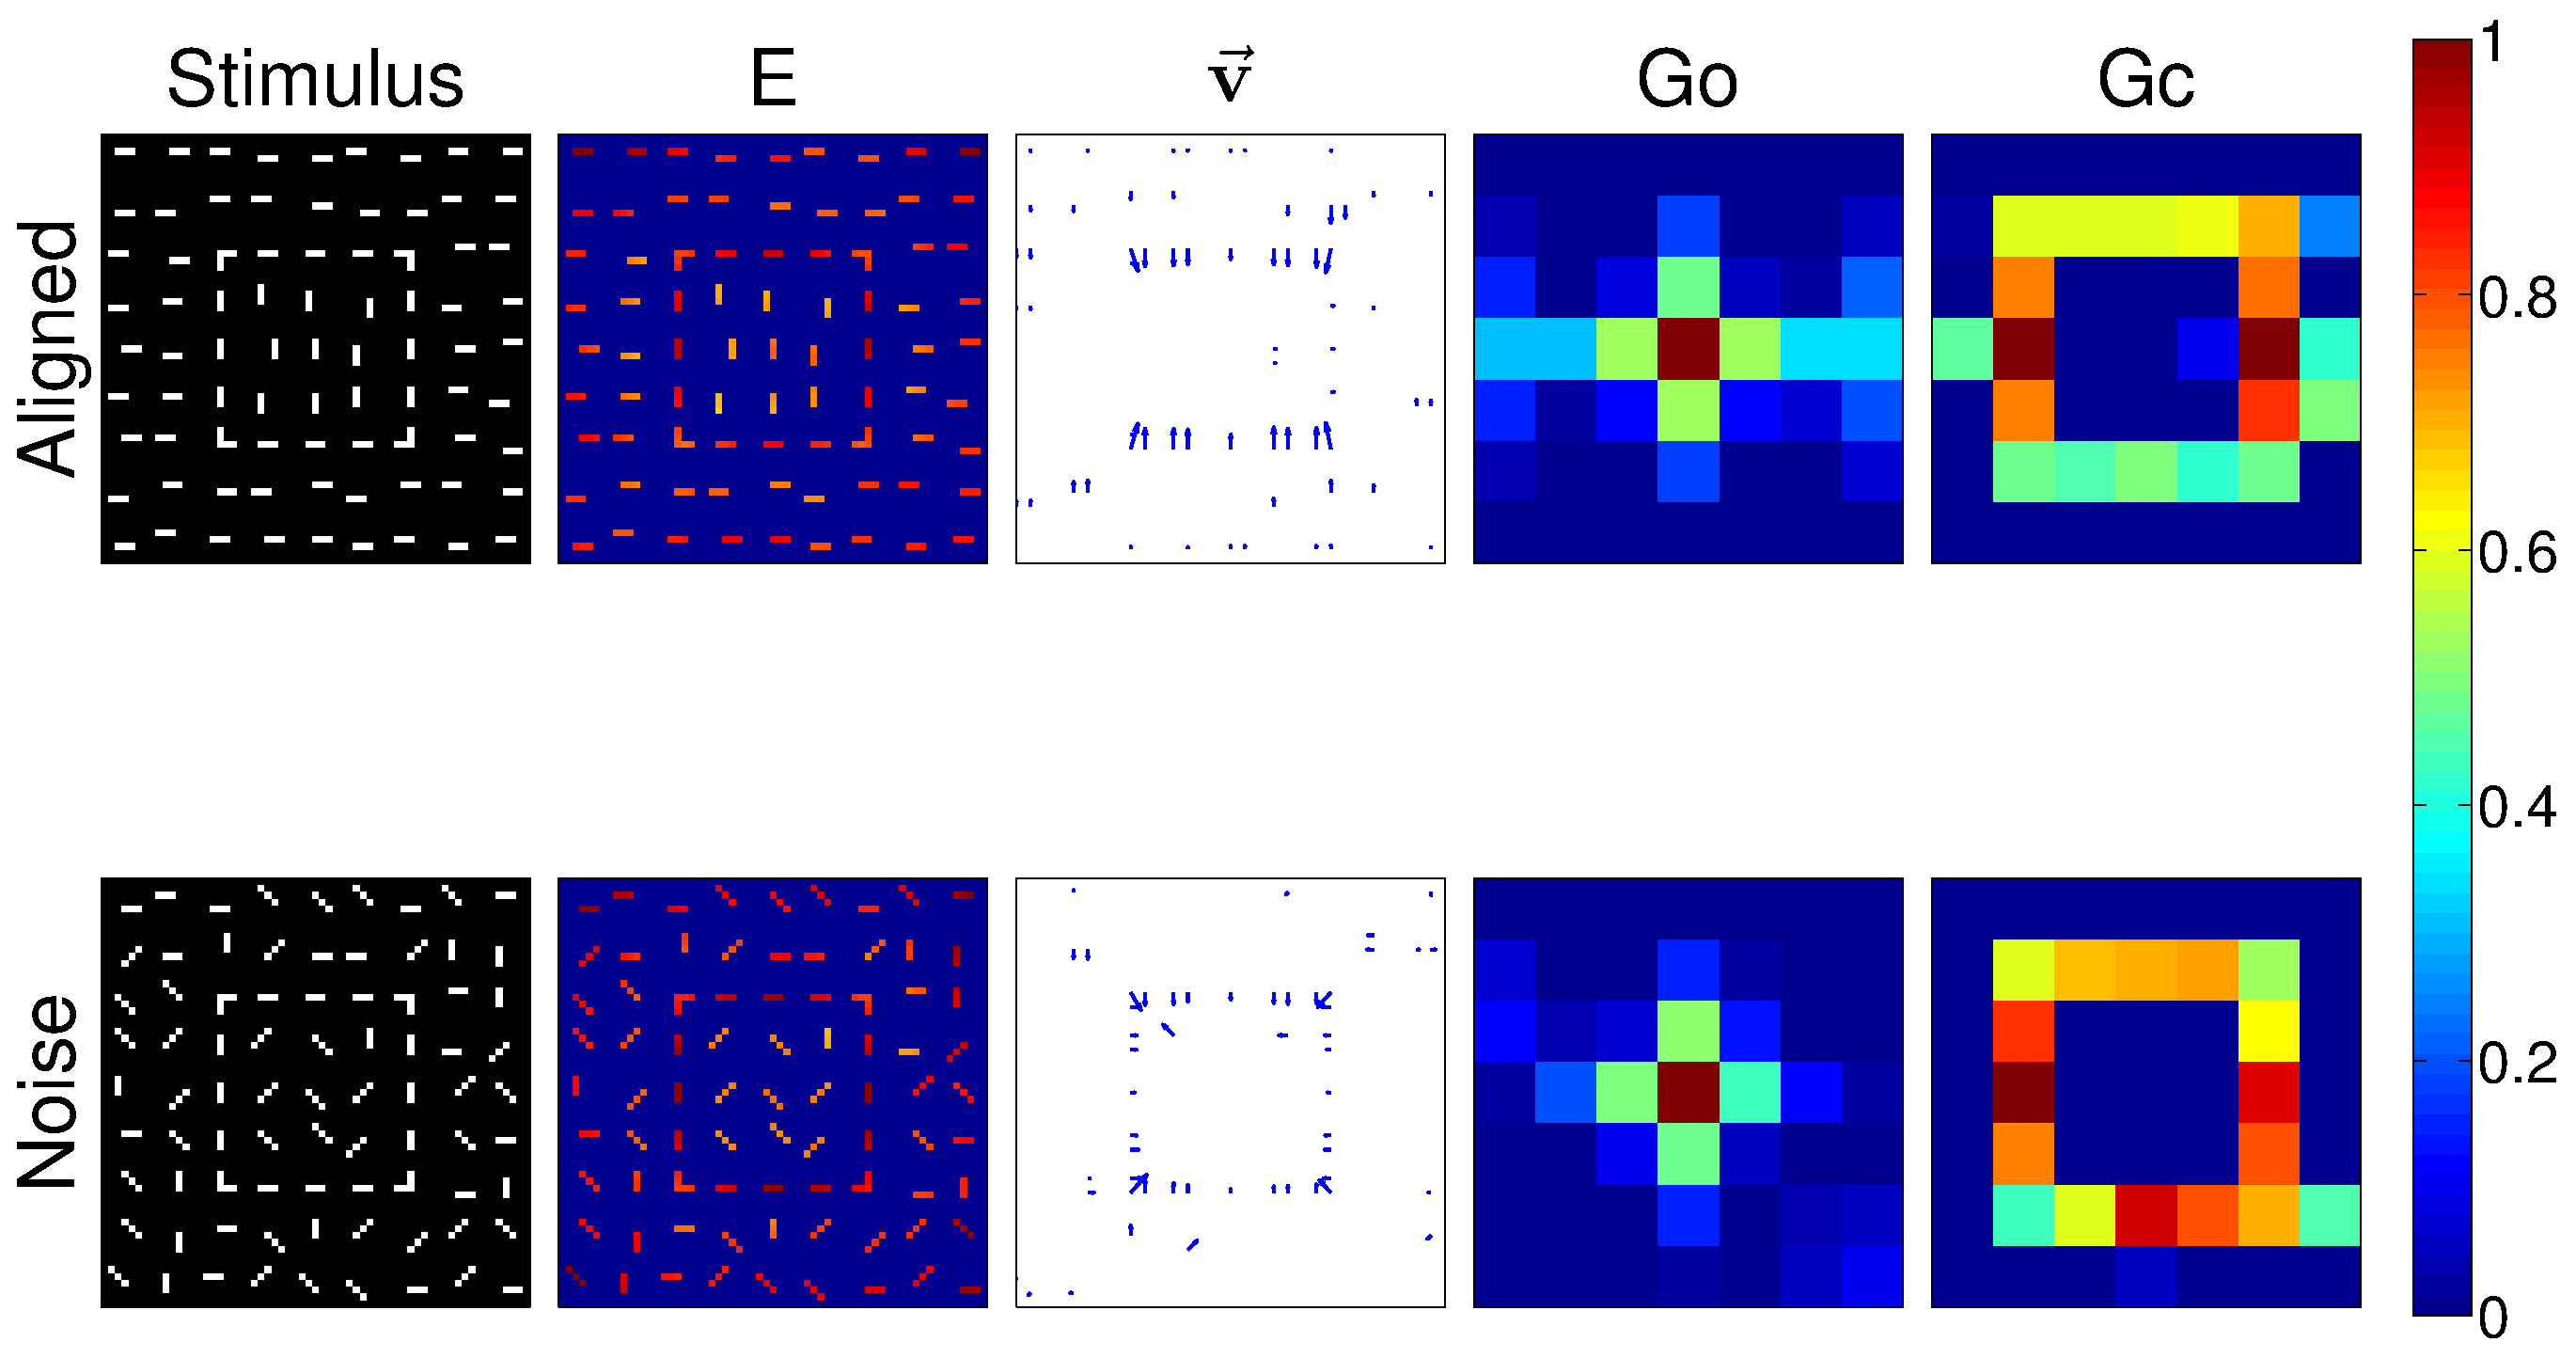
\includegraphics[width=0.75\textwidth]{Fig7.eps}
\end{center}
\caption{Figure-ground segregation of a square object with aligned contour elements (top
  row) and with noise contour elements (top row). Shown are (left to right) the input
  stimulus, the edge cell activity (E), the border ownership
  assignment along edges (shown as the vector modulation index 
  $\protect\vv{\mathbf{v}}$,
  section~\ref{sec:vmi}), the object grouping 
  neuron activity 
$(G_o)$
 and the contour grouping activity
$(G_c)$.
 Activities are normalized within each map, and warmer colors
  indicate higher activity (see color bar at right).}
\label{Fig:Square_Noise}
\end{figure*}

\subsection{Interaction between border ownership assignment and attention} 
\label{sec:BOS-att}

Although border ownership selectivity emerges independently of
attention~\citep{Qiu_etal07}, attention may help to facilitate
figure-ground segregation in the presence of noise.
 For the square figure with noise, we found that 
in our model, attention increases the responses of neurons
along the edge of the figure (unpaired t-test, $p=\num{2.32e-59}$) and
suppresses those in the center (unpaired t-test,
$p=\num{3.42e-8}$). In addition, attention increases border-ownership
modulation along the edge of the figure (unpaired t-test,
$p=\num{1.37e-143}$) and increases the activity of object grouping
neurons in the center of the figure (unpaired t-test,
$p=\num{1.53e-239}$). All effects were small but highly significant,
and were based on the differences in summed activity of neurons along
the edge or center of the figure over a total of 100 simulations.
Figure~\ref{Fig:Attention_modulation} shows the average neural
activity in the different populations of neurons in our model, with
and without the effect of attention.  

Attention must also operate in cluttered environments where multiple
objects may be present. \cite{Qiu_etal07} studied border-ownership
responses in area V2 when two overlapping squares were presented and
attention was directed either to the foreground or background
square. \cite{Mihalas_etal11b}, using a model closely related to ours
but without $G_c$ cells, reproduced the experimental
finding that border-ownership modulation was strong when attention was
on the foreground figure but weak when attention was on the background
figure. Our model reproduces this finding, see Supplementary Figure
\ref{Fig:Overlap_Square}. The quantitative effect on border-ownership
selectivity is shown in Figure~\ref{Fig:Overlap_Square_exp_model}. 
Our model also reproduces the experimental 
finding that border-ownership modulation is strong when attention is
on the foreground figure (Figure~\ref{Fig:Overlap_Square_exp_model}C,
``Front attended") and weak when attention is on the background
figure (Figure~\ref{Fig:Overlap_Square_exp_model}C, ``Back attended").

These results demonstrate that the object and contour grouping neurons
are able to assist with early level segmentation of objects in noise
and clutter.  Previous experimental studies have only tested squares
without noise, although the effect of figures defined by broken
contours has been investigated before~\citep{Zhang_vonderHeydt10}.
Our results predict that border ownership assignment and grouping are
robust even in the presence of noise,  clutter, and interruptions in figure borders, 
and that attention may further aid this process.

\begin{figure*}[t]
\begin{center}
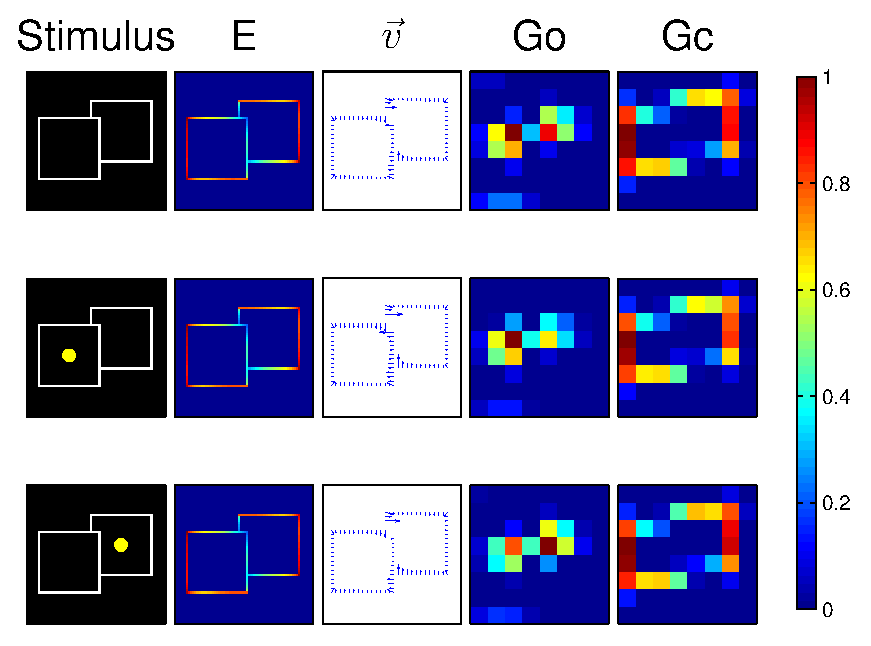
\includegraphics[width=\textwidth]{Fig8.eps}
\end{center}
\caption{Attentional modulation of different neuronal populations aids figure-ground segregation in the presence of noise. Each panel (A-D) shows the means and standard deviations of neural activity with and without added attention over 100 different simulations. (A) Edge cell activity along the contour of the object shows enhancement with attention. (B) Edge cell activity in the center of the figure shows suppression with attention. (C) The BOS signal along the contour of the object shows enhancement with attention. (D) Object grouping cell (Go) activity centered on the object shows enhancement with attention}
\label{Fig:Attention_modulation}
\end{figure*}


\section{Discussion}
\label{sec:discussion}

In this study, we use computational models to elucidate the role of
attention and feedback in contour and object processing. Different
from many models that are tailor-made to reproduce one set of experimental
results, we demanded that our model explain data
from at least three sets of experimental approaches, (1)~contour
integration, (2)~figure-ground segregation, (3)~attention to objects.  
We hypothesize that these processes are fundamentally linked in terms of the larger
goal of image understanding.  Using the same set of model parameters,
we reproduced several experimental findings and generated non-trivial
predictions. 

\subsection{Model predictions}
Our model predicts that attentional modulation is specific to the
attended contour or object, rather than being defined purely
spatially. This is possible because, in our model, attention modifies
firing rates of grouping cells, rather than of elementary
feature-coding cells. Attending to the contour increases
contour-response $d'$ in both V1 and V4, consistent with experimental
results showing increased contour-related responses after animals had
been trained to perform a contour detection task, compared to when
they performed a separate set of tasks in which the contour was
behaviorally irrelevant~\citep{Li_etal08a}. We note that
\cite{Li_etal08a} only studied neural responses in V1, while our model
makes predictions about attention-related changes to contour-response
$d'$ in both V1 and V4.  We also find that attention modulates border
ownership activity in V2 in an object-based manner. As a result, our
model makes predictions about neural activity in visual areas V1, V2,
and V4 across different stimuli and tasks.

We predict that the interaction of modulatory feedback from grouping
cells with local inhibition enhances the representation of the figure
and suppresses the representation of the background.  Indeed, our
model produces background suppression for isolated contours as well as
for figures embedded in noise.  We note that this prediction is
different from what others have observed in texture-defined figures
\citep{Lamme95,Lee_etal98a}, where there is generally response
enhancement of the center of the figure.  This difference may be due
to how the figure is defined, by its contour in our experiment and by
texture in \cite{Lamme95} and \cite{Lee_etal98a}.
It is possible that if feedback from object grouping neurons is to the center of the
figure instead of its edges, we may observe enhancement of activity at
the center of the figure. Understanding how border-ownership
assignment interacts with filling-in of surfaces is a future direction
of research.  Furthermore we predict that attention, in addition to
enhancing the figure in an object-based manner, also helps to suppress
noise in the background.

We also predict that removing feedback from V4 to lower visual areas
reduces neural responses in V1, while having a smaller effect in V4.
The activity of V4 neurons is also affected due to the recurrency of
the network model. This could be tested experimentally by the same contour
detection task used by~\cite{Chen_etal14}, and measuring the
contour-response $d'$ in V1 and V4 from reversible inactivation of
feedback connections. Although complete and selective deactivation of
V4 feedback to areas V1 and/or V2 is technically challenging, there
have been attempts to study the effect of this type of feedback either
through extra-striate lesions~\citep{Super_Lamme07} or reversible
inactivation~\citep{Jansen-Amorim_etal12}.  Anesthesia presumably also
decreases top-down influences, and indeed reduces contour-related V1
responses \citep{Li_etal08a} and figure-ground segregation
\citep{Lamme_etal98}.

\begin{figure*}[t]
\begin{center}
\includegraphics[width=0.75\textwidth]{Fig9.eps}
\end{center}
\caption{Quantitative comparison of model performance to
  neurophysiological findings \citep{Qiu_etal07} for border-ownership coding of
  overlapping figures. (A) The stimulus configurations used are shown,
  with neurons coding right border ownership (black) and left border
  ownership (gray) when attention was focused on either foreground
  square 1 (front attended) or on background square 2 (back
  attended). (B) The responses of border ownership selective cells
  recorded in V2 are shown:  bars indicate the
  average firing rate 
  for each stimulus condition. (C) Model B cell responses to analogous
  stimulus conditions. For both the model and the experiments,
  border-ownership modulation was strong when attention was on
  foreground but weak when attention was on background. 
Panels~A and~B are modified from Figure~3 of~\cite{Qiu_etal07}.} 
\label{Fig:Overlap_Square_exp_model}
\end{figure*}

\subsection{Comparison to other models}

Many have argued that contour integration and figure-ground
segregation are largely local phenomena that rely on lateral
connections \citep{Grossberg94, Grossberg97, Li98, Zhaoping05,
  Piech_etal13}.  While some of these models include a role for top-down
influences \citep{Li98,Piech_etal13}, they do not offer a specific
mechanism by which higher visual areas representing object-level
information selectively feed back to lower visual areas containing
feature-level information about the object.  In contrast, our model is
explicit in that feedback connections from higher visual areas
modulate the responses of early feature-selective neurons involved in
the related processes of contour integration and figure-ground
segregation. Our model thus is a member of a broad class of theoretical models that achieve image
understanding through bottom-up and top-down recurrent
processing~\citep{Ullman84,Hochstein_Ahissar02,Roelfsema_06,Epshtein_etal08}.
In comparison to similar models, our model is able to reproduce
experimental findings from two traditionally separate fields of
study-- contour integration and figure-ground assignment. Importantly,
using the same set of network parameters, the grouping cells in our
model are able to represent proto-objects (both contours and extended
objects) and provide a perceptual organization of the scene. We 
show that this perceptual organization is critical for interfacing with top-down
attention, and that it provides a general theoretical framework for
understanding how feedback connections and an hierarchy of visual
areas can be used to group together the features of an object. 

\subsection{Roles of V1 and V4 in visual processing}

While V1 neurons have small RFs that accurately code for orientation, V1 also shows strong background inhibition off the contour. This property allows V1 neurons
to enhance contours and suppress noise in the image at a high spatial
resolution. V4 neurons, on the other hand, have large RFs that integrate
local feature information over large areas of visual space and provide
a coarse, proto-object representation of contours and objects.
Feedback from V4 can then be refined by the lateral connections present
within early visual areas, which aids in the enhancement of the figure
and its edges in the image.

Even when V1 neurons receive no feedback from V4, there is an
increase in contour-response $d'$ with contour length
(Figure~\ref{Fig:FB_att}). This contour facilitation is solely due to
the excitatory lateral connections present in V1, and is weaker
without feedback. As a result, feedback from V4 may not be necessary
for contour facilitation, but it interacts with local lateral
connections in a push-pull manner -- neurons along the contour are
enhanced, while elements on the background are suppressed. Not
surprisingly, removing this type of feedback has a larger effect on V1
neurons compared to V4 neurons, although the activity of V4 neurons is
also affected due to the recurrency of the network model.

\subsection{Contour and object grouping neurons}

Contour grouping neurons have direct experimental support through the
recent neurophysiological experiments published by \cite{Chen_etal14}.
In our model, relatively few numbers of grouping neurons (both contour
and object) are required. The spatial resolution of the grouping
process does not need to be very high, as grouping cells only provide
a coarse template of the contours and objects present in the
scene. Assuming that the activity of grouping cells represents
proto-objects with a similar resolution as attention, the total number
of grouping cells may be less than 2\% of the number of
border-ownership cells~\citep{Craft_etal07}. 
In the contour integration experiments~\citep{Chen_etal14}, many V4
neurons were found to respond to straight, elongated contours, while
in our model, only a subset of the grouping neurons are selective for
contours. One possible explanation for this is overtraining -- monkeys
performed the task a very large number of times
each day for many months, and
neural plasticity may have generated many V4 neurons
which respond to contours. 

There is no unambiguous neurophysiological evidence for object grouping
neurons yet, although previous studies have found neurons in V4 that
respond to contour segments of various
curvatures~\citep{Pasupathy_Connor02,Brincat_Connor04}. The receptive
fields of these neurons are similar to those proposed
 by \cite{Craft_etal07}. Other types of grouping neurons may also exist,
including those that respond to gratings~\citep{Hegde_vanEssen07},
illusory surfaces~\citep{Cox_etal13}, or 3D
surfaces~\citep{He_Nakayama95,Hu_etal15a}.  We do not attempt to model
the whole array of grouping neurons that may exist, but only those
necessary for reproducing the neurophysiological experiments referred
to here.

In our model, orientation-independent attentional input to contour
grouping cells was used to enhance neural responses to a contour at a
given location.  We note that this form of attention is analogous to
the size- and location tolerant attentional selection process proposed
by~\cite{Mihalas_etal11b}. The local circuitry of their model was able
to sharpen a relatively broad and nonspecific attentional input to
match the size and location of a figure in the visual
scene. Similarly, the local circuitry of our model transforms the
orientation-independent attentional input such that it only enhances
the contour of the correct orientation. We note that attention also has a suppressive effect in our model, essentially inhibiting unattended objects and locations. 
There is physiological support for this mechanism~\citep{Wegener_etal04,Hopf_etal06,Sundberg_etal09,Tsotsos11}. Furthermore, previous results show
suppression of border-ownership activity along the shared edge of
overlapping squares when the back square was attended, but not the
front square~\citep{Qiu_etal07}. Finally, psychophysical
experiments demonstrate an ``object superiority effect,'' where
reaction times are fastest when attention is directed to targets that
are part of the cued object, and slowest when targets are outside of
an object~\citep{Egly_etal94,Kimchi_etal07}. 

Complementarily, feature-based attention acts broadly across the
visual scene and increases the responses of all components that share
similar feature attributes (\eg color, orientation, or direction of
movement) with the attended
component \citep{Motter94a,Treue_Trujillo99}.
Orientation-specific forms of attention
can enhance neural
responses in V1 and V4, but do not significantly alter
tuning curves or selectivity~\citep{McAdams_Maunsell99a}. 
Our model may be able to reproduce similar results by essentially changing the
form of the attentional input to be orientation-specific, \ie top-down
attention targets a \emph{single} population of contour grouping
neurons with the same orientation preference.
We expect that both
object-based and feature-based forms of attention exist and can be
flexibly used for different tasks.

\subsection{Scope and limitations of the model}
Our model seeks to reproduce two different sets of experimental
results, while making testable predictions for future experiments. 
We only included one scale of grouping neurons for
simplicity, although 
multiple scales of grouping
neurons are needed to account for the diversity in the scale of
objects in the real world.
Our model also assigns distinct roles to the
different visual areas,  edge processing in V1, border ownership
assignment in V2, and grouping of contours and objects in V4. However,
the physiological properties of neurons in early visual areas have not
been fully characterized, and 
neurons in these different
areas may have 
additional ranges of selectivity
than the ones we assign them in our model. 
Finally, our model operates on artificial
images composed of simple shapes such as contours or square
figures. In order to truly understand grouping mechanisms in natural
vision, our model must also be able to operate on natural images as
input, where the number of potential objects and features are much
richer. We are currently working  
on the construction of such a model.

\begin{acknowledgements}
We would like to thank Justin Killebrew for his help
in using the computational cluster in order to run the simulations. We would also
like to thank R\"udiger von der Heydt for sharing his deep insights on
vision with us. 
\end{acknowledgements}

\section*{Compliance with Ethical Standards}
\subsection*{Conflict of interest}
The authors declare that they have no conflict of
interest.

% BibTeX users please use one of
%\bibliographystyle{spbasic}      % basic style, author-year citations
%%\bibliographystyle{spmpsci}      % mathematics and physical sciences
%%\bibliographystyle{spphys}       % APS-like style for physics
%\bibliography{niebase,niebase_supp}   % name your BibTeX data base

%%%% Non-BibTeX users please use
\begin{thebibliography}{90}
\providecommand{\natexlab}[1]{#1}
\providecommand{\url}[1]{{#1}}
\providecommand{\urlprefix}{URL }
\expandafter\ifx\csname urlstyle\endcsname\relax
  \providecommand{\doi}[1]{DOI~\discretionary{}{}{}#1}\else
  \providecommand{\doi}{DOI~\discretionary{}{}{}\begingroup
  \urlstyle{rm}\Url}\fi
\providecommand{\eprint}[2][]{\url{#2}}

\bibitem[{Ardila et~al(2012)Ardila, Mihalas, von~der Heydt, and
  Niebur}]{Ardila_etal12}
Ardila D, Mihalas S, von~der Heydt R, Niebur E (2012) {M}edial axis generation
  in a model of perceptual organization. In: IEEE CISS-2012 46th Annual
  Conference on Information Sciences and Systems, IEEE, Princeton University,
  NJ, pp 1--4

\bibitem[{Baek and Sajda(2005)}]{Baek_Sajda05}
Baek K, Sajda P (2005) {I}nferring figure-ground using a recurrent
  integrate-and-fire neural circuit. IEEE Transactions on Neural Systems and
  Rehabilitation Engineering 13(2):125--130

\bibitem[{Bosking et~al(1997)Bosking, Zhang, Schofield, and
  Fitzpatrick}]{Bosking_etal97}
Bosking WH, Zhang Y, Schofield B, Fitzpatrick D (1997) {O}rientation
  selectivity and the arrangement of horizontal connections in tree shrew
  striate cortex. The Journal of Neuroscience 17(6):2112--2127

\bibitem[{Brincat and Connor(2004)}]{Brincat_Connor04}
Brincat S, Connor C (2004) {U}nderlying principles of visual shape selectivity
  in posterior inferotemporal cortex. Nature Neuroscience 7:880--886

\bibitem[{Chen et~al(2014)Chen, Yan, Gong, Gilbert, Liang, and
  Li}]{Chen_etal14}
Chen M, Yan Y, Gong X, Gilbert CD, Liang H, Li W (2014) {I}ncremental
  integration of global contours through interplay between visual cortical
  areas. Neuron 82(3):682--694

\bibitem[{Cox et~al(2013)Cox, Schmid, Peters, Saunders, Leopold, and
  Maier}]{Cox_etal13}
Cox MA, Schmid MC, Peters AJ, Saunders RC, Leopold DA, Maier A (2013)
  {R}eceptive field focus of visual area {V}4 neurons determines responses to
  illusory surfaces. Proceedings of the National Academy of Sciences
  110(42):17,095--17,100

\bibitem[{Craft et~al(2007)Craft, Sch{\"u}tze, Niebur, and von~der
  Heydt}]{Craft_etal07}
Craft E, Sch{\"u}tze H, Niebur E, von~der Heydt R (2007) {A} neural model of
  figure-ground organization. Journal of Neurophysiology 97(6):4310--26, pMID:
  17442769

\bibitem[{Domijan and {\v{S}}eti{\'c}(2008)}]{Domijan_Setic08}
Domijan D, {\v{S}}eti{\'c} M (2008) A feedback model of figure-ground
  assignment. Journal of Vision 8(7):10--10

\bibitem[{Dong et~al(2008)Dong, Mihalas, Qiu, von~der Heydt, and
  Niebur}]{Dong_etal08a}
Dong Y, Mihalas S, Qiu F, von~der Heydt R, Niebur E (2008) {S}ynchrony and the
  binding problem in macaque visual cortex. Journal of {V}ision 8(7):1--16,
  \urlprefix\url{http://journalofvision.org/8/7/30/, doi:10.1167/8.7.30},
  pMC2647779

\bibitem[{Duncan(1984)}]{Duncan84}
Duncan J (1984) {Selective attention and the organization of visual
  information}. J Exp Psychol Gen 113:501--517

\bibitem[{Egly et~al(1994)Egly, Driver, and Rafal}]{Egly_etal94}
Egly R, Driver J, Rafal R (1994) {S}hifting visual attention between objects
  and locations: evidence for normal and parietal lesion subjects. Journal of
  Experimental Psychology: General 123:161--77

\bibitem[{Epshtein et~al(2008)Epshtein, Lifshitz, and Ullman}]{Epshtein_etal08}
Epshtein B, Lifshitz I, Ullman S (2008) {I}mage interpretation by a single
  bottom-up top-down cycle. Proceedings of the National Academy of Sciences
  105(38):14,298--14,303

\bibitem[{Field et~al(1993)Field, Hayes, and Hess}]{Field_etal93}
Field DJ, Hayes A, Hess RF (1993) {C}ontour integration by the human visual
  system: evidence for a local association field. Vision Research
  33(2):173--193

\bibitem[{Gilbert and Wiesel(1989)}]{Gilbert_Wiesel89}
Gilbert C, Wiesel T (1989) {C}olumnar specificity of intrinsic horizontal and
  cortico- cortical connections in cat visual cortex. J Neurosci 9:2432--2442

\bibitem[{Girard et~al(2001)Girard, Hup\'{e}, and Bullier}]{Girard_etal01}
Girard P, Hup\'{e} J, Bullier J (2001) {F}eedforward and feedback connections
  between areas {V}1 and {V}2 of the monkey have similar rapid conduction
  velocities. J Neurophysiol 85:1328--1331

\bibitem[{Gray et~al(1989)Gray, {K\"onig}, Engel, and Singer}]{Gray_etal89}
Gray C, {K\"onig} P, Engel A, Singer W (1989) {O}scillatory responses in cat
  visual cortx exhibit inter-columnar synchronization which reflects global
  stimulus properties. Nature 338:334--337

\bibitem[{Green and Swets(1966)}]{Green_Swets66}
Green DM, Swets JA (1966) {S}ignal {D}etection {T}heory and {P}sychophysics.
  Wiley, New York, N.Y.

\bibitem[{Grossberg(1994)}]{Grossberg94}
Grossberg S (1994) {3-D} vision and figure-ground separation by visual cortex.
  Perception \& Psychophysics 55:48--120

\bibitem[{Grossberg(1997)}]{Grossberg97}
Grossberg S (1997) {C}ortical dynamics of three-dimensional figure--ground
  perception of two-dimensional pictures. Psychological review 104(3):618,
  pMID: 9243966

\bibitem[{He and Nakayama(1995)}]{He_Nakayama95}
He ZJ, Nakayama K (1995) {V}isual attention to surfaces in three-dimensional
  space. Proc Natl Acad Sci U S A 9(24):11,155--11,159, pMID: 7479956

\bibitem[{Hegd{\'e} and Van~Essen(2007)}]{Hegde_vanEssen07}
Hegd{\'e} J, Van~Essen DC (2007) {A} comparative study of shape representation
  in macaque visual areas {V}2 and {V}4. Cerebral Cortex 17(5):1100--1116

\bibitem[{Hesse and Tsao(2016)}]{Hesse_Tsao16}
Hesse JK, Tsao DY (2016) Consistency of border-ownership cells across
  artificial stimuli, natural stimuli, and stimuli with ambiguous contours.
  Journal of Neuroscience 36(44):11,338--11,349

\bibitem[{von~der Heydt et~al(2003)von~der Heydt, Qiu, and
  He}]{vonderHeydt_etal03a}
von~der Heydt R, Qiu FT, He ZJ (2003) {N}eural mechanisms in border ownership
  assignment: motion parallax and gestalt cues. J Vision 3(9):666a

\bibitem[{Ho and Yeh(2009)}]{Ho_Yeh09}
Ho MC, Yeh SL (2009) {E}ffects of instantaneous object input and past
  experience on object-based attention. Acta psychologica 132(1):31--39

\bibitem[{Hochstein and Ahissar(2002)}]{Hochstein_Ahissar02}
Hochstein S, Ahissar M (2002) {V}iew from the top: {H}ierarchies and reverse
  hierarchies in the visual system. Neuron 36(5):791--804

\bibitem[{Hopf et~al(2006)Hopf, Boehler, Luck, Tsotsos, Heinze, and
  Schoenfeld}]{Hopf_etal06}
Hopf J, Boehler C, Luck S, Tsotsos J, Heinze H, Schoenfeld M (2006) {Direct
  neurophysiological evidence for spatial suppression surrounding the focus of
  attention in vision}. Proceedings of the National Academy of Sciences
  103(4):1053, pMID: 16410356

\bibitem[{Hu et~al(2015)Hu, von~der Heydt, and Niebur}]{Hu_etal15a}
Hu B, von~der Heydt R, Niebur E (2015) {A} neural model for perceptual
  organization of 3{D} surfaces. In: IEEE CISS-2015 49th Annual Conference on
  Information Sciences and Systems, IEEE Information Theory Society, Baltimore,
  MD, pp 1--6, \doi{10.1109/CISS.2015.7086906}

\bibitem[{Hup\'{e} et~al(1998)Hup\'{e}, James, Payne, Lomber, Girard, and
  Bullier}]{Hupe_etal98}
Hup\'{e} J, James A, Payne B, Lomber S, Girard P, Bullier J (1998) {C}ortical
  feedback improves discrimination between figure and background by {V}1, {V}2
  and {V}3 neurons. Nature 394:784--787

\bibitem[{Intriligator and Cavanagh(2001)}]{Intriligator_Cavanagh01}
Intriligator J, Cavanagh P (2001) {T}he spatial resolution of visual attention.
  Cognit Psychol 43:171--216

\bibitem[{Jansen-Amorim et~al(2012)Jansen-Amorim, Fiorani, and
  Gattass}]{Jansen-Amorim_etal12}
Jansen-Amorim AK, Fiorani M, Gattass R (2012) {GABA} inactivation of area {V}4
  changes receptive-field properties of {V}2 neurons in {C}ebus monkeys.
  Experimental {N}eurology 235(2):553--562

\bibitem[{Jehee et~al(2007)Jehee, Lamme, and Roelfsema}]{Jehee_etal07b}
Jehee JF, Lamme VA, Roelfsema PR (2007) Boundary assignment in a recurrent
  network architecture. Vision research 47(9):1153--1165

\bibitem[{Kikuchi and Akashi(2001)}]{Kikuchi_Akashi01}
Kikuchi M, Akashi Y (2001) {A} model of border-ownership coding in early
  vision. In: Dorffner G, Bischof H, Hornik K (eds) ICANN 2001, pp 1069--74

\bibitem[{Kimchi et~al(2007)Kimchi, Yeshurun, and
  Cohen-Savransky}]{Kimchi_etal07}
Kimchi R, Yeshurun Y, Cohen-Savransky A (2007) {A}utomatic, stimulus-driven
  attentional capture by objecthood. Psychon Bull Rev 14(1):166--172

\bibitem[{Koffka(1935)}]{Koffka35}
Koffka K (1935) {P}rinciples of {G}estalt psychology. Harcourt-Brace, New York

\bibitem[{Kreiter and Singer(1992)}]{Kreiter_Singer92}
Kreiter AK, Singer W (1992) {O}scillatory neuronal responses in the visual
  cortex of the awake macaque monkey. Europ J Neurosci 4(4):369--375

\bibitem[{Lamme(1995)}]{Lamme95}
Lamme VAF (1995) {T}he neurophysiology of figure-ground segregation in primary
  visual cortex. J Neurosci 15:1605--1615

\bibitem[{Lamme et~al(1998)Lamme, Zipser, and Spekreijse}]{Lamme_etal98}
Lamme VAF, Zipser K, Spekreijse H (1998) {F}igure-ground activity in primary
  visual cortex is suppressed by anesthesia. Proc Natl Acad Sci U S A
  9(6):3263--3268

\bibitem[{Layton et~al(2012)Layton, Mingolla, and Yazdanbakhsh}]{Layton_etal12}
Layton OW, Mingolla E, Yazdanbakhsh A (2012) {D}ynamic coding of
  border-ownership in visual cortex. Journal of vision 12(13):8

\bibitem[{Lee et~al(1998)Lee, Mumford, Romero, and Lamme}]{Lee_etal98a}
Lee TS, Mumford D, Romero R, Lamme VAF (1998) {T}he {R}ole of the {P}rimary
  {V}isual {C}ortex in {H}igher {L}evel {V}ision. Vision Research 38:2429--2452

\bibitem[{Li et~al(2008)Li, Pi{\"e}ch, and Gilbert}]{Li_etal08a}
Li W, Pi{\"e}ch V, Gilbert CD (2008) {L}earning to link visual contours. Neuron
  57(3):442--451

\bibitem[{Li(1998)}]{Li98}
Li Z (1998) {A} {N}eural {M}odel of {C}ontour {I}ntegration in the {P}rimary
  {V}isual {C}ortex. Neural Computation 10(903-940)

\bibitem[{Martin and von~der Heydt(2015)}]{Martin_vonderHeydt15}
Martin AB, von~der Heydt R (2015) {S}pike {S}ynchrony {R}eveals {E}mergence of
  {P}roto-{O}bjects in {V}isual {C}ortex. The Journal of Neuroscience
  35(17):6860--6870

\bibitem[{McAdams and Maunsell(1999)}]{McAdams_Maunsell99a}
McAdams CJ, Maunsell JHR (1999) {E}ffects of attention on orientation-tuning
  functions of single neurons in macaque cortical area {V}4. J Neurosci
  19:431--441

\bibitem[{Mihalas et~al(2011)Mihalas, Dong, von~der Heydt, and
  Niebur}]{Mihalas_etal11b}
Mihalas S, Dong Y, von~der Heydt R, Niebur E (2011) {M}echanisms of perceptual
  organization provide auto-zoom and auto-localization for attention to
  objects. Proceedings of the National Academy of Sciences 108(18):7583--8,
  pMC3088583

\bibitem[{Motter(1994)}]{Motter94a}
Motter BC (1994) {N}eural correlates of attentive selection for color or
  luminance in extrastriate area {V4}. J Neurosci 14:2178--2189

\bibitem[{Nishimura and Sakai(2004)}]{Nishimura_Sakai04}
Nishimura H, Sakai K (2004) {D}etermination of border-ownership based on the
  surround context of contrast. Neurocomputing 58-60:843--8

\bibitem[{Nishimura and Sakai(2005)}]{Nishimura_Sakai05}
Nishimura H, Sakai K (2005) {T}he computational model for border-ownership
  determination consisting of surrounding suppression and facilitation in early
  vision. Neurocomputing 65:77--83

\bibitem[{de~Oliveira et~al(1997)de~Oliveira, Thiele, and
  Hoffmann}]{DeOliveira_etal97}
de~Oliveira SC, Thiele A, Hoffmann KP (1997) {S}ynchronization of neuronal
  activity during stimulus expectation in a direction discrimination task. J
  Neurosci 17(23):9248--60

\bibitem[{Pao et~al(1999)Pao, Geiger, and Rubin}]{Pao_etal99}
Pao HK, Geiger D, Rubin N (1999) {M}easuring convexity for {F}igure/{G}round
  {S}eparation. In: 7th International Conference on Computer Vision, Kerkyra,
  Greece

\bibitem[{Pasupathy and Connor(2002)}]{Pasupathy_Connor02}
Pasupathy A, Connor CE (2002) {P}opulation coding of shape in area {V}4. Nature
  neuroscience 5(12):1332--1338

\bibitem[{Pi{\"e}ch et~al(2013)Pi{\"e}ch, Li, Reeke, and
  Gilbert}]{Piech_etal13}
Pi{\"e}ch V, Li W, Reeke GN, Gilbert CD (2013) {N}etwork model of top-down
  influences on local gain and contextual interactions in visual cortex.
  Proceedings of the National Academy of Sciences 110(43):E4108--E4117,
  pMC3808648

\bibitem[{Polat et~al(1998)Polat, Mizobe, Pettet, Kasamatsu, and
  Norcia}]{Polat_etal98}
Polat U, Mizobe K, Pettet MW, Kasamatsu T, Norcia AM (1998) {C}ollinear
  {S}timuli {R}egulate {V}isual {R}esponses {D}epending on {C}ell's {C}ontrast
  {T}hreshold. Nature 391:580--584

\bibitem[{Poort et~al(2012)Poort, Raudies, Wannig, Lamme, Neumann, and
  Roelfsema}]{Poort_etal12}
Poort J, Raudies F, Wannig A, Lamme VA, Neumann H, Roelfsema PR (2012) {T}he
  role of attention in figure-ground segregation in areas {V1} and {V4} of the
  visual cortex. Neuron 75(1):143--156

\bibitem[{Qiu and von~der Heydt(2005)}]{Qiu_vonderHeydt05}
Qiu FT, von~der Heydt R (2005) {F}igure and ground in the visual cortex: {V}2
  combines stereoscopic cues with {G}estalt rules. Neuron 47:155--166

\bibitem[{Qiu and von~der Heydt(2007)}]{Qiu_vonderHeydt07}
Qiu FT, von~der Heydt R (2007) {N}eural representation of transparent overlay.
  Nat Neurosci 10(3):283--284

\bibitem[{Qiu et~al(2007)Qiu, Sugihara, and von~der Heydt}]{Qiu_etal07}
Qiu FT, Sugihara T, von~der Heydt R (2007) {F}igure-ground mechanisms provide
  structure for selective attention. Nat Neurosci 10(11):1492--9

\bibitem[{Rensink(2000)}]{Rensink00a}
Rensink RA (2000) {T}he dynamic representation of scenes. Visual Cognition
  7(1/2/3):17--42

\bibitem[{Roelfsema(2006)}]{Roelfsema_06}
Roelfsema PR (2006) {C}ortical algorithms for perceptual grouping. Annu Rev
  Neurosci 29:203--227

\bibitem[{Roelfsema et~al(2004)Roelfsema, Lamme, and
  Spekreijse}]{Roelfsema_etal04}
Roelfsema PR, Lamme VAF, Spekreijse H (2004) {S}ynchrony and covariation of
  firing rates in the primary visual cortex during contour grouping. Nat
  Neurosci 7(9):982--991, \doi{10.1038/nn1304},
  \urlprefix\url{http://dx.doi.org/10.1038/nn1304}

\bibitem[{Russell et~al(2014)Russell, Mihalas, von~der Heydt, Niebur, and
  Etienne-Cummings}]{Russell_etal14}
Russell AF, Mihalas S, von~der Heydt R, Niebur E, Etienne-Cummings R (2014) {A}
  model of proto-object based saliency. Vision Research 94:1--15

\bibitem[{Sajda and Finkel(1995)}]{Sajda_Finkel95}
Sajda P, Finkel L (1995) {I}ntermediate-{L}evel {V}isual {R}epresentations and
  the {C}onstruction of {S}urface {P}erception. J Cogn Neurosci 7:267--291

\bibitem[{Sakai et~al(2012)Sakai, Nishimura, Shimizu, and Kondo}]{Sakai_etal12}
Sakai K, Nishimura H, Shimizu R, Kondo K (2012) Consistent and robust
  determination of border ownership based on asymmetric surrounding contrast.
  Neural Networks 33:257--274

\bibitem[{Scholl(2001)}]{Scholl01}
Scholl BJ (2001) {O}bjects and attention: the state of the art. Cognition
  80(1-2):1--46

\bibitem[{Sch{\"u}tze et~al(2003)Sch{\"u}tze, Niebur, and von~der
  Heydt}]{Schutze_etal03}
Sch{\"u}tze H, Niebur E, von~der Heydt R (2003) {M}odeling cortical mechanisms
  of border ownership coding. J Vision 3(9):114a

\bibitem[{Singer(1999)}]{Singer99b}
Singer W (1999) {N}euronal synchrony: a versatile code for the definition of
  relations? Neuron 24:49--65

\bibitem[{Stemmler et~al(1995)Stemmler, Usher, and Niebur}]{Stemmler_etal95a}
Stemmler M, Usher M, Niebur E (1995) {L}ateral cortical connections may
  contribute to both contour completion and redundancy reduction in visual
  processing. Soc Neurosci Abstr 21(1):510

\bibitem[{Stettler et~al(2002)Stettler, Das, Bennett, and
  Gilbert}]{Stettler_etal02}
Stettler DD, Das A, Bennett J, Gilbert CD (2002) {L}ateral connectivity and
  contextual interactions in macaque primary visual cortex. Neuron
  36(4):739--750

\bibitem[{Sugihara et~al(2011)Sugihara, Qiu, and von~der
  Heydt}]{Sugihara_etal11}
Sugihara T, Qiu FT, von~der Heydt R (2011) {T}he speed of context integration
  in the visual cortex. Journal of neurophysiology 106(1):374--385, pMC3129740

\bibitem[{Sundberg et~al(2009)Sundberg, Mitchell, and
  Reynolds}]{Sundberg_etal09}
Sundberg KA, Mitchell JF, Reynolds JH (2009) {Spatial attention modulates
  center-surround interactions in macaque visual area v4}. Neuron 61:952--963

\bibitem[{Sup{\`e}r and Lamme(2007)}]{Super_Lamme07}
Sup{\`e}r H, Lamme VA (2007) {A}ltered figure-ground perception in monkeys with
  an extra-striate lesion. Neuropsychologia 45(14):3329--3334

\bibitem[{Thiele and Stoner(2003)}]{Thiele_Stoner03}
Thiele A, Stoner G (2003) {N}euronal synchrony does not correlate with motion
  coherence in cortical area {MT}. Nature 421(6921):366--370

\bibitem[{Treisman(1996)}]{Treisman96b}
Treisman A (1996) {T}he binding problem. Curr Opin Neurobiol 6(2):171--178

\bibitem[{Treue(1999)}]{Treue_Trujillo99}
Treue JCM Sand~Trujillo (1999) {F}eature-based attention influences motion
  processing gain in macaque visual cortex. Nature 399:575--9

\bibitem[{Treue(2001)}]{Treue01}
Treue S (2001) {N}eural correlates of attention in primate visual cortex.
  Trends in Neurosciences 24:295--300

\bibitem[{Tschechne and Neumann(2014)}]{Tschechne_Neumann14}
Tschechne S, Neumann H (2014) Hierarchical representation of shapes in visual
  cortex—from localized features to figural shape segregation. Frontiers in
  computational neuroscience 8:93

\bibitem[{Tsotsos(2011)}]{Tsotsos11}
Tsotsos JK (2011) A Computational Perspective on Visual Attention. MIT Press

\bibitem[{Ullman(1984)}]{Ullman84}
Ullman S (1984) {V}isual routines. Cognition 18:97--159

\bibitem[{Ullman et~al(1992)Ullman, Gregory, and Atkinson}]{Ullman92}
Ullman S, Gregory R, Atkinson J (1992) {L}ow-{L}evel {A}spects of
  {S}egmentation and {R}ecognition [and {D}iscussion]. Philosophical
  Transactions of the Royal Society of London Series B: Biological Sciences
  337(1281):371--379

\bibitem[{Ungerleider et~al(2007)Ungerleider, Galkin, Desimone, and
  Gattass}]{Ungerleider_etal07}
Ungerleider LG, Galkin TW, Desimone R, Gattass R (2007) {C}ortical connections
  of area {V}4 in the macaque. Cerebral Cortex 18(3):477--499

\bibitem[{Wagatsuma et~al(2016)Wagatsuma, von~der Heydt, and
  Niebur}]{Wagatsuma_etal16a}
Wagatsuma N, von~der Heydt R, Niebur E (2016) {S}pike {S}ynchrony {G}enerated
  by {M}odulatory {C}ommon {I}nput through {NMDA}-type {S}ynapses. Journal of
  Neurophysiology 116(3):1418--1433

\bibitem[{Wegener et~al(2004)Wegener, Freiwald, and Kreiter}]{Wegener_etal04}
Wegener D, Freiwald WA, Kreiter AK (2004) The influence of sustained selective
  attention on stimulus selectivity in macaque visual area mt. Journal of
  Neuroscience 24(27):6106--6114

\bibitem[{Wertheimer(1923)}]{Wertheimer23}
Wertheimer M (1923) {U}ntersuchungen zur {Lehre von der Gestalt II}. Psychol
  Forsch 4:301--350

\bibitem[{Williford and von~der Heydt(2013)}]{Williford_vonderHeydt13}
Williford JR, von~der Heydt R (2013) {B}order-ownership coding. Scholarpedia
  8(10):30,040

\bibitem[{Williford and von~der Heydt(2014)}]{Williford_vonderHeydt14}
Williford JR, von~der Heydt R (2014) {E}arly {V}isual {C}ortex {A}ssigns
  {B}order {O}wnership in {N}atural {S}cenes {A}ccording to {I}mage {C}ontext.
  Journal of Vision 14(10):588--588

\bibitem[{Yen and Finkel(1998)}]{Yen_Finkel98}
Yen SC, Finkel LH (1998) {E}xtraction of perceptually salient contours by
  striate cortical networks. Vision research 38(5):719--741

\bibitem[{Zeki(1978)}]{Zeki78b}
Zeki SM (1978) {U}niformity and diversity of structure and function in rhesus
  monkey prestriate visual cortex. The Journal of Physiology 277(1):273--290

\bibitem[{Zhang and von~der Heydt(2010)}]{Zhang_vonderHeydt10}
Zhang N, von~der Heydt R (2010) {A}nalysis of the context integration
  mechanisms underlying figure--ground organization in the visual cortex. The
  Journal of Neuroscience 30(19):6482--6496, pMC2910339

\bibitem[{Zhaoping(2005)}]{Zhaoping05}
Zhaoping L (2005) {B}order ownership from intracortical interactions in visual
  area {V2}. Neuron 47:143--153, pMID: 15996554

\bibitem[{Zhou et~al(2000)Zhou, Friedman, and von~der Heydt}]{Zhou_etal00}
Zhou H, Friedman HS, von~der Heydt R (2000) {C}oding of border ownership in
  monkey visual cortex. J Neurosci 20(17):6594--6611, pMID: 10964965

\bibitem[{Zwickel et~al(2007)Zwickel, Wachtler, and Eckhorn}]{Zwickel_etal07}
Zwickel T, Wachtler T, Eckhorn R (2007) Coding the presence of visual objects
  in a recurrent neural network of visual cortex. Biosystems 89(1):216--226

\end{thebibliography}

\clearpage

%en do you say anywhere that you put the code on github?
%bh added one sentence at the beginning giving the link

\onecolumn
\appendix
\pagenumbering{arabic} % restart page numbering in appendix
\renewcommand\theequation{S\arabic{equation}}    
\setcounter{equation}{0}  
\renewcommand{\thefigure}{S\arabic{figure}} % add S before figures
\setcounter{figure}{0}  % reset figure count here
\section*{Supplementary Material}
\subsection*{Details of Model Implementation}
\label{sec:appendix}
%bh added
The source code for this paper can be found online at:
https://github.com/brianhhu/Contour\_BOS.
%
 One pixel in our model input represents the typical size of the receptive
field for 
a V1
edge cell (which at eccentricity 5 $\deg$ is about 0.7
$\deg$, Chen {\em et al}. 2014).  The simulated visual field is
assumed to be homogeneous
(\ie, we neglect the influence of the cortical magnification factor).  
Each neuronal unit in the model represents multiple
neurons with overlapping receptive fields and similar tuning.  It is
referred to as a ``neuron'' in the following and it is represented by
an ordinary differential equation, eq.~1.  For all examples the system
is simulated for 0.5s and an equilibrium is reached within a few tens
or about hundred simulated ms.  A typical simulation of a visual field of
$64\times 64$ units consists of 30,528 coupled ordinary differential
equations which are solved using a fourth-order Runge-Kutta  algorithm
in MATLAB.

Each neuron is characterized by its spatial location, its type (edge
cell, object grouping cell, \etc) and one additional property, as
follows. E cells are indexed by the angle of their preferred
orientation: $0$, $\pi/4$, $\pi/2$, and $3\pi/4$
(all angles relative to the horizontal). 
B cells are indexed
by the angle of their preferred side of figure: right, $0$; upper
right, $\pi/4$; up, $\pi/2$; upper left, $3\pi/4$; left, $\pi$; lower
left, $5\pi/4$; down, $3\pi/2$; lower right, $7\pi/4$. 
Note that the preferred side of a 
B~cell
 is always orthogonal to its preferred orientation. Contour
grouping cells are indexed by their preferred orientation ($0$,
$\pi/4$, $\pi/2$, and $3\pi/4$), while object grouping neurons are
selective for annuli of a preferred radius.
As discussed earlier, we only use one preferred radius in this model,
which we chose as corresponding to 16 pixels in the input layer.
The network receives two types
of inputs. A binary edge map activates E~cells, taking value 1 if an
edge of that orientation is present
at this location in the image and (-1)
otherwise. Finally, an attentional field stimulates grouping cells,
with maximal strength of 0.07. This value is listed in
Table~\ref{partable}, as are those of all other model parameters.

In the following, we define the anatomical connection patterns between
all neuronal populations in our model. Obviously, this defines the
receptive (and projective) fields of all model neurons. At the input
level, edge cells ($E$ population)  receive 
one-to-one
connections from input units
($IN$ population) of the respective preferred
orientations $o_i$ at 
position $(x,y)$,
resulting in
a connectivity weight distribution as follows,
\begin{align}
	WIN^{o_1}_{x,y}E^{o_2}_{x,y}=
	\begin{cases}
	intoe_w \:\;&if\;o_1 = o_2\\\nonumber
	-1\;&otherwise
	\end{cases}\\
\end{align}
where the weight of the input to edge cell connections, $intoe_w$ is a
scaling parameter, and its value is set to 1.  Changing it does not
produce different activation patterns in the network but rather scales
up all activities.
This is indicated in Table~\ref{partable} by an asterisk (*) next to
the value of this parameter, as well as to that of all others with
this property.

The connections from edge cells 
to inhibitory IE cells are two-dimensional isotropic Gaussians: 

\begin{align}
	&WE_{x_1,y_1}IE_{x_2,y_2}=N_{etoie}\: \exp\left(-\frac{(x_1-x_2)^2}{2\: etoie_{sd}^2}-\frac{(y_1-y_2)^2}{2\: etoie_{sd}^2}\right)\
\end{align}
where the normalization coefficient $N_{etoie}$ is determined from:
\begin{align}
	etoie_w = \sum^{24}_{i,j=-24} WE_{x,y}IE_{x+i,y+j}
\label{eq:normalizationetoie}
\end{align}

The weight of the edge to IE connections $etoie_w$ is set to 8. The standard deviation of the lateral connections,
$etoie_{sd}$ was chosen to be eight times the size of the edge cells'
receptive field size. For simplicity, all lateral connections in V1
are assumed to have the same standard deviation.
The upper limit in the sum of eq.~\ref{eq:normalizationetoie} is where
we truncate the Gaussian distribution used to define the
connectivities, at three times its standard deviation (8), equal to 24
times the size of a V1 RF.

IE cells are not orientation selective, and inhibit all edge cells in
their neighborhood. The strength of inhibition is independent of
the preferred orientation of the edge cells and has the same
pattern as the reciprocal edge to IE cell connections: 
\begin{align}
	&WIE_{x_1,y_1}E_{x_2,y_2}=N_{ietoe}\: \exp\left(-\frac{(x_1-x_2)^2}{2\: ietoe_{sd}^2}-\frac{(y_1-y_2)^2}{2\: ietoe_{sd}^2}\right)\
\end{align}
where the normalization coefficient $N_{ietoe}$ is determined from:
\begin{align}
	ietoe_w = \sum^{24}_{i,j=-24} WIE_{x,y}E_{x+i,y+j}
\end{align}

The strength of the inhibitory connections IE to edge cells,
$ietoe_w$, is an important parameter in the model. Its value was
chosen to be -8, which is just strong enough for the inhibition of the
edge cells to cancel out activity in the case of a uniform stimulation
field. In our model, attention in the absence of edges is a broad
field, and experimental observations show little effect of attention
alone on the firing rates of purely sensory (edge) cells.
E cells locally connect to other edge cells of the same preferred
orientation. These connections allow for the passing of contour
information along a line. The connection weights are,
\begin{align}
	WE^{o_1}_{x_1,y_1}E^{o_2}_{x_2,y_2}&=N_{etoe}\: \delta_{o_1,o_2}\: \delta_{y_1,0}\: \delta_{y_2,0}\:
	\exp\left(-\frac{(x_1-x_2)^2}{2\: etoe_{sd} ^2}\right)\ {\rm
          if}\ o_1,o_2 = 0 \nonumber\\
	WE^{o_1}_{x_1,y_1}E^{o_2}_{x_2,y_2}&=N_{etoe}\: \delta_{o_1,o_2}\: \delta_{x_1,y_1}\: \delta_{x_2,y_2}\: 
	\exp\left(-\frac{(x_1-x_2)^2}{2\: etoe_{sd} ^2}\right)\  {\rm
          if}\ o_1,o_2 = \pi/4 \nonumber\\
	WE^{o_1}_{x_1,y_1}E^{o_2}_{x_2,y_2}&=N_{etoe}\: \delta_{o_1,o_2}\: \delta_{x_1,0}\: \delta_{x_2,0}\:
	\exp\left(-\frac{(y_1-y_2)^2}{2\: etoe_{sd} ^2}\right)\  {\rm
          if}\ o_1,o_2 = \pi/2 \nonumber\\
	WE^{o_1}_{x_1,y_1}E^{o_2}_{x_2,y_2}&=N_{etoe}\: \delta_{o_1,o_2}\: \delta_{x_1,-y_1}\: \delta_{x_2,-y_2}\: 
	\exp\left(-\frac{(y_1-y_2)^2}{2\: etoe_{sd} ^2}\right)\  {\rm
          if}\ o_1,o_2 = 3\pi/4 \nonumber\\
\end{align}
where the normalization coefficient $N_{etoe}$ is determined from:
\begin{align}
	etoe_w = \sum^{24}_{i,j=-24} WE^{o}_{x,y}E^{o}_{x+i,y+j}
\end{align}

The weight of the excitatory lateral connections $etoe_w=2/3$ is
chosen such that individual excitatory connections are stronger than
the nonspecific inhibitory connections for a line of cells along the
preferred direction, 
and that the integral of the excitatory connections is smaller than
the integral of the inhibitory ones. The standard deviation
$etoe_{sd}=8$ is the same as for all other lateral connections in V1.  

The edge cells E excite a pair of border-ownership cells with the same
preferred orientation $o_1$
and at the same position, $(x_i,y_i)$.  Border ownership selective
cells have opposite 
side-of-figure preferences
$o_2$ which are orthogonal to $o_1$
(\ie differing by $\pi/2$ in either direction).
They are generated by
connections from E cells whose  weight is given by  a 2D Gaussian, 
\begin{align}
	WE^{o_1}_{x_1,y_1}B^{o_2}_{x_2,y_2}&=etob_w \:	\exp\left(-\frac{(x_1-x_2)^2}{2\: etob_{sd} ^2}-\frac{(y_1-y_2)^2}{2\: etob_{sd} ^2}\right)\ \nonumber\\
	%&\sin^2(o_1-o_2) = 1 \nonumber\\
	o_1&\in \left\{0,\pi/4,\pi/2,3\pi/4 \right\} \nonumber\\
	o_2&\in \left\{0,\pi/4,\pi/2,3\pi/4,\pi,5\pi/4,3\pi/2,7\pi/4\ \right\} \nonumber\\
\end{align}
where the weight of the E to border-ownership connections, $etob_w$ is set to 1.

The connections from border-ownership to inhibitory IB cells are two-dimensional Gaussians: 
\begin{align}
	&WB_{x_1,y_1}IB_{x_2,y_2}=N_{btoib}\: \exp\left(-\frac{(x_1-x_2)^2}{2\: btoib_{sd}^2}-\frac{(y_1-y_2)^2}{2\: btoib_{sd}^2}\right)\
\end{align}
where the normalization coefficient $N_{btoib}$ is determined from:
\begin{align}
	btoib_w = \sum^{12}_{i,j=-12} WB_{x,y}IB_{x+i,y+j}
\end{align}

The weight of the border-ownership to IB connections $btoib_w$ is set to 2. The standard deviation of the lateral connections,
$btoib_{sd}$ was chosen to be four times the size of the border-ownership cells' receptive field size. For simplicity, all lateral connections in V2 are assumed to have the same standard deviation.

IB cells, which are not orientation selective, inhibit all border-ownership in their neighborhood with the same pattern as B to IB cell excitation:
\begin{align}
	&WIB_{x_1,y_1}B_{x_2,y_2}=N_{ibtob}\: \exp\left(-\frac{(x_1-x_2)^2}{2\: ibtob_{sd}^2}-\frac{(y_1-y_2)^2}{2\: ibtob_{sd}^2}\right)\
\end{align}
where the normalization coefficients $N_{ibtob}$ is determined from:
\begin{align}
	ibtob_w = \sum^{12}_{i,j=-12} WIB_{x,y}B_{x+i,y+j}
\end{align}

The strength of the inhibitory connections IB to border-ownership, $ibtob_w$, is an important parameter in the
model. Its value was chosen to be -2, which is just strong enough for
the inhibition of the border-ownership cells to 
cancel out activity
in the case of a uniform stimulation field. In our model, attention in the absence of edges is a broad field, and experimental observations show little effect of attention alone on the firing rates of border-ownership cells. This parameter also influences the value of the attention modulation of the non-preferred border ownership cells, and the value which was a
priori chosen reproduces well the observed experimental value.

B cells connect to other border-ownership cells of the same preferred
side of figure. These connections allow the passing of border
ownership signal along a line: 
\begin{align}
	WB^{o_1}_{x_1,y_1}B^{o_2}_{x_2,y_2}&=N_{btob}\: \delta_{o_1,o_2}\: \delta_{x_1,0}\: \delta_{x_1,0}\: 
	\exp\left(-\frac{(y_1-y_2)^2}{2\: btob_{sd} ^2}\right)\  o_1,o_2\in \left\{0,\pi\right\}\nonumber\\
	WB^{o_1}_{x_1,y_1}B^{o_2}_{y_2,y_2}&=N_{btob}\: \delta_{o_1,o_2}\: \delta_{x_1,-y_1}\: \delta_{x_2,-y_2}\:
	\exp\left(-\frac{(y_1-y_2)^2}{2\: etoe_{sd} ^2}\right)\  o_1,o_2\in \left\{\pi/4,5\pi/4 \right\}\nonumber\\
	WB^{o_1}_{x_1,y_1}B^{o_2}_{x_2,y_2}&=N_{btob}\: \delta_{o_1,o_2}\: \delta_{y_1,0}\: \delta_{y_2,0}\: 
	\exp\left(-\frac{(x_1-x_2)^2}{2\: btob_{sd} ^2}\right)\ o_1,o_2\in \left\{\pi/2,3\pi/2 \right\}\nonumber\\
	WB^{o_1}_{x_1,y_1}B^{o_2}_{x_2,y_2}&=N_{btob}\: \delta_{o_1,o_2}\: \delta_{x_1,y_1}\: \delta_{x_2,y_2}\: 
	\exp\left(-\frac{(x_1-x_2)^2}{2\: btob_{sd} ^2}\right)\  o_1,o_2\in \left\{3\pi/4,7\pi/4 \right\}	
\end{align}
where the normalization coefficient $N_{btob}$ is determined from:
\begin{align}
	btob_w = \sum^{12}_{i,j=-12} WB^{o}_{x,y}B^{o}_{x+i,y+j}
\end{align}

The weight of the excitatory lateral connections $btob_w=2/3$ is
chosen such that individual excitatory connections are stronger than
the nonspecific inhibitory connections for a line of cells along the
preferred direction, 
and that the integral of the excitatory connections is smaller than
the integral of the inhibitory ones. The standard deviation
$btob_{sd}=4$ is the same as for all other lateral connections in V2.  

B cells also connect to other border-ownership cells of orthogonal preferred
orientation. These connections allow the passing of border ownership
information along a corner, where rot is a rotation operator that rotates the connection matrix $C_f$ by the angle $o$:
\begin{align}
	WB^{o_1}_{x_1,y_1}B^{o_2}_{x_2,y_2}&=btob_{wc}\: (\text{rot}_{o_1}(C_f(x_2-x_1,y_2-y_1)) \delta_{o_1,o_2-\pi/2} \\\nonumber
	&+c\:\text{rot}_{o_1+\pi}(C_f(x_2-x_1,y_2-y_1)) \delta_{o_1,o_2-\pi/2} \\\nonumber
	&+\text{rot}_{o_2}(C_b(x_2-x_1,y_2-y_1)) \delta_{o_1,o_2+\pi/2} \\\nonumber
	&+c\:\text{rot}_{o_2+\pi}(C_b(x_2-x_1,y_2-y_1)) \delta_{o_1,o_2+\pi/2} )
\end{align}
with the matrices
\begin{align}
	C_f(x,y)=
	\begin{cases}
	N_{btobc}\;\exp(-\frac{x^2+y^2}{2\:btob_{sd}^2})\;&if\;x\geq0\:\&\:y<0\\
	0\;&otherwise
	\end{cases}\\
	C_b(x,y)=
	\begin{cases}
	N_{btobc}\;\exp(-\frac{x^2+y^2}{2\:btob_{sd}^2})\;&if\;x\geq0\:\&\:y>0\\
	0\;&otherwise
	\end{cases}
\end{align}
and the normalization coefficient $N_{btobc}$ is obtained from
\begin{align}
1=\sum^{12}_{i,j=-12} C_f(i,j)
\end{align}
The values of $btob_{wc}=2/3$ and $c=2/3$ were chosen to be the same as $btob_w$.

The connections from border-ownership cells to object grouping cells consist of 2D Gaussians rotated to the appropriate angle and arranged in a circular fashion, 
where $btogo_{sds}$ and $btog_{sdl}$ are the spreads of the Gaussian in the radial and tangential directions, respectively:
\begin{align}
	WB^{o}_{x_1,y_1}G^{r}_{x_2,y_2}&=\text{rot}_{o}\left(N_{btogr}\: \exp\left(-\frac{(x_1-x_2+r)^2}{2\: (btogo_{sds} r)^2}
	-\frac{(y_1-y_2)^2}{2\: (btog_{sdl} r)^2}\right)\right)\  \nonumber\\  
	o&\in \left\{0,\pi/4,\pi/2,3\pi/4,\pi,5\pi/4,3\pi/2,7\pi/4\right\} \nonumber\\
\end{align}
where the normalization coefficient $N_{btogr}$ is
\begin{align}
	btog_w=\sum^{2r}_{i=-2r} WB^{0}_{x-r,y+i}G^{r}_{x,y}
\end{align}

The strength of the border-ownership to grouping connections $btog_w$,
is a scaling parameter and was chosen to be 0.125, since in the model
there are 4 preferred orientations and two side-of-figure preferences
(8 total orientations)
for the border-ownership cells,
each of which sends input to each grouping cell.
 Each orientation of
border-ownership cells provides a 2D Gaussian input to the grouping
cells, with the standard deviation on the direction orthogonal to the
radius being 0.5 times the radius, while the standard deviation on the
direction parallel to the radius is 0.25 times the radius. (If these
standard deviations are too large, then grouping cells lose
specificity and, for more complicated images, some edges are assigned
incorrectly. If these standard deviations are too small, the density
of grouping cells needs to be increased.) The distance between two
neighboring cells of radius $r$ is $r/2$, such that a line is never
more than one standard deviation away from the center of a patch of
connections involved in its grouping.

The feedback from the object grouping cells to lower level feature-selective neurons follows a similar spatial pattern of the
B to object grouping connections. The feedback to E and B are similar,  except E cells receive feedback with twice the radius and standard deviations to account for upsampling to twice the number of neurons in the V1 layer:
\begin{align}
	WG^{r}_{x_2,y_2}B^{o_1}_{x_1,y_1}&=\text{rot}_{o_1}\left(N_{gtobr}\: \exp\left(-\frac{(x_1-x_2+r)^2}{2\: (btogo_{sds} r)^2}
	-\frac{(y_1-y_2)^2}{2\: (btog_{sdl} r)^2}\right)\right)\ \nonumber\\ 
	WG^{r}_{x_2,y_2}E^{o_2}_{x_1,y_1}&=\text{rot}_{o_2+\pi/2}\left(N_{gtoer}\: \exp\left(-\frac{(x_1-x_2+(2r))^2}{2\: (btogo_{sds} (2r))^2}
		-\frac{(y_1-y_2)^2}{2\: (btog_{sdl} (2r))^2}\right)\right)\nonumber\\
		&+\text{rot}_{o_2+3\pi/2}\left(N_{gtoer}\: \exp\left(-\frac{(x_1-x_2+(2r))^2}{2\: (btogo_{sds} (2r))^2}
				-\frac{(y_1-y_2)^2}{2\: (btog_{sdl} (2r))^2}\right)\right)\ \nonumber\\ o_1&\in \left\{0,\pi/4,\pi/2,3\pi/4,\pi,5\pi/4,3\pi/2,7\pi/4\ \right\} \nonumber\\
		o_2&\in \left\{0,\pi/4,\pi/2,3\pi/4 \right\} \nonumber\\
\end{align}
Since the number of the grouping cells on a line is
inverse proportional to their scale, the line integral of the weight
is considered proportional to the radius of the G cell: 

\begin{align}
	gtob_w=\sum^{2r}_{i=-2r} WG^{r}_{x,y}B^{\pi}_{x+r,y+i}
\end{align}

The value of $gtob_w=2/3$ is critical for the model, and the border ownership modulation index depends critically on it. In order to reproduce the observed attention modulation of the nonpreferred side of figure for B cells, the weight of the feedback to edge cells needs to be four times that to the border ownership cells $gtoe_w=8/3$.

In previous work~\citep{Mihalas_etal11b},
 in order to fit the observed reaction time cost observed when irelevant objects are outside the focus of attention, a feedback
from G to IG cells is introduced. Here, this connection allows for competition between different grouping neurons. This has the same pattern, but half the scaled weight as the
feedback to B cells and twice its standard deviations: 
\begin{align}
	WG^{r}_{x_2,y_2}IG^{o}_{x_1,y_1}&=\text{rot}_{o}\left(N_{gtobr}\: \exp\left(-\frac{(x_1-x_2+r)^2}{2\: (btogo_{sds} (2r))^2}
	-\frac{(y_1-y_2)^2}{2\: (btog_{sdl} (2r))^2}\right)\right) \  \nonumber\\ o&\in \left\{0,\pi/4,\pi/2,3\pi/4,\pi,5\pi/4,3\pi/2,7\pi/4\ \right\} \nonumber\\
\end{align}

The connections from inhibitory IG cells to object grouping cells follow a similar connection pattern as the B to G cell excitation, except with the antipreferred orientation inhibiting the G cells:
\begin{align}
  WIG^{o+\pi}_{x_1,y_1}G^{r}_{x_2,y_2}&=\text{rot}_{o+\pi}\left(N_{igtogr}\:
        \exp\left(-\frac{(x_1-x_2+r)^2}{2\: (btogo_{sds} r)^2}
                -\frac{(y_1-y_2)^2}{2\: (btog_{sdl} r)^2}\right)\right) \nonumber\\ \ o&\in \left\{0,\pi/4,\pi/2,3\pi/4,\pi,5\pi/4,3\pi/2,7\pi/4\ \right\} \nonumber\\
\end{align}
with the normalization coefficient $N_{igtogr}$  obtained from:
\begin{align}
	igtog_w&=\sum^{2r}_{i=-2r} WIG^{\pi}_{x-r,y+i}G^{r}_{x,y} 	
\end{align}
as well as inhibition from orthogonal orientations:
\begin{align}
	W_{o}IG^{o\pm\pi/2}_{x_1,y_1}G^{r}_{x_2,y_2}&=\text{rot}_{o\pm\pi/2}\left(N_{igtogro}\: \exp\left(-\frac{(x_1-x_2+r)^2}{2\: (btogo_{sds} r)^2}
        -\frac{(y_1-y_2)^2}{2\: (btog_{sdl} r)^2}\right)\right)\ \nonumber\\ o&\in
        \left\{0,\pi/4,\pi/2,3\pi/4,\pi,5\pi/4,3\pi/2,7\pi/4\ \right\} \nonumber\\ 
\end{align}
with the normalization coefficient $N_{igtogro}$ obtained from:
\begin{align}
	igtog_{wo}&=\sum^{2r}_{i=-2r} W_{o}IG^{\pi/2}_{x-r,y+i}G^{r}_{x,y} 	
\end{align}

It is assumed that the strength of the inhibition from the nonpreferred
side of figure $igtog_w$ is equal to that of orthogonal preferred sides
of figures $igtog_{wo}$, and each of them is equal to the value of the
excitatory strength $btog_w$. Similar to the lateral connections in
V2, this feedback loop has stronger but fewer and more specific
excitatory connections, resulting in robust activity for specific
inputs and more total inhibitory connection weights, resulting in
little activity cased by nonspecific inputs. 

Similarly, the connections from border-ownership cells with opposite side of figure preferences to contour grouping cells with the same preferred orientation consist of rotated 2D Gaussians,
where $btogc_{sds}$ and $btog_{sdl}$ are the spreads of the Gaussian in the radial and tangential directions, respectively:

\begin{align}
	WB^{o_1}_{x_1,y_1}G^{o_2}_{x_2,y_2}&=\text{rot}_{o_1}\left(N_{btogr}\: \exp\left(-\frac{(x_1-x_2)^2}{2\: (btogc_{sds} r)^2}
	-\frac{(y_1-y_2)^2}{2\: (btog_{sdl} r)^2}\right)\right)\  \nonumber\\ 
	 &\sin^2(o_1-o_2) = 1 \nonumber\\
	 o_1&\in \left\{0,\pi/4,\pi/2,3\pi/4,\pi,5\pi/4,3\pi/2,7\pi/4\ \right\} \nonumber\\
	 o_2&\in \left\{0,\pi/4,\pi/2,3\pi/4 \right\} \nonumber\\
\end{align}
where the normalization coefficient $N_{btogr}$ is chosen such that
\begin{align}
	btog_w=\sum^{2r}_{i=-2r} WB^{0}_{x,y+i}G^{0}_{x,y}
\end{align}

There is also excitation from other orientations, in order to explain the orientation dependence
of V4 neurons:
\begin{align}
	W_{o}B^{o_1}_{x_1,y_1}G^{o_2}_{x_2,y_2}&=\frac{3}{4}\: \text{rot}_{o_1}\left(N_{btogo}\: \exp\left(-\frac{(x_1-x_2)^2}{2\: (btogc_{sds} r)^2}
        -\frac{(y_1-y_2)^2}{2\: (btog_{sdl} r)^2}\right)\right)\ \nonumber\\
        	 &\sin^2(o_1-o_2) = \frac{\sqrt{2}}{2} \nonumber\\
    W_{o}B^{o_1}_{x_1,y_1}G^{o_2}_{x_2,y_2}&=\frac{1}{4}\: \text{rot}_{o_1}\left(N_{btogo}\: \exp\left(-\frac{(x_1-x_2)^2}{2\: (btogc_{sds} r)^2}
        -\frac{(y_1-y_2)^2}{2\: (btog_{sdl} r)^2}\right)\right)\ \nonumber\\
        	 &\sin^2(o_1-o_2) = 0 \nonumber\\
	 o_1&\in \left\{0,\pi/4,\pi/2,3\pi/4,\pi,5\pi/4,3\pi/2,7\pi/4\ \right\} \nonumber\\
	 o_2&\in \left\{0,\pi/4,\pi/2,3\pi/4 \right\} \nonumber\\
\end{align}
with the normalization coefficient $N_{btogo}$ obtained from:
\begin{align}
	btog_{wo}&=\sum^{2r}_{i=-2r} WB^{0}_{x,y+i}G^{0}_{x,y} 	
\end{align}

The strength of the border-ownership to grouping connections $btog_w$,
is a scaling parameter and was chosen to be 0.125, since in the model
there are 4 preferred orientations and two side-of-figure preferences
(8 total orientations) for the border-ownership cells,
each of which sends input to each grouping cell. Each orientation of
border-ownership cells provides a 2D Gaussian input to the grouping
cells, with the standard deviation on the direction orthogonal to the
radius being 0.5 times the radius, while the standard deviation on the
direction parallel to the radius is 0.1 times the radius. This standard deviation parallel to the radius is smaller than that for object grouping neurons (0.25 times the radius) to account for higher selectivity to contours.

The feedback from the grouping cells also follows the spatial pattern of the B to grouping connections. The feedback to E and B are similar, although E cells receive feedback with twice the standard deviations to account for the higher number of neurons in the V1 layer:
\begin{align}
	WG^{o_1}_{x_2,y_2}B^{o_2}_{x_1,y_1}&=\text{rot}_{o_2}\left(N_{gtobr}\: \exp\left(-\frac{(x_1-x_2)^2}{2\: (btogc_{sds} r)^2}
	-\frac{(y_1-y_2)^2}{2\: (btog_{sdl} r)^2}\right)\right)\ \nonumber\\
		        	 &\sin^2(o_1-o_2) = 1 \nonumber\\
	WG^{o_1}_{x_2,y_2}E^{o_1}_{x_1,y_1}&=\text{rot}_{o_1}\left(N_{gtobr}\: \exp\left(-\frac{(x_1-x_2)^2}{2\: (btogc_{sds} (2r))^2}
	-\frac{(y_1-y_2)^2}{2\: (btog_{sdl} (2r))^2}\right)\right)\ \nonumber\\ 
		 o_1&\in \left\{0,\pi/4,\pi/2,3\pi/4 \right\} \nonumber\\
	 o_2&\in \left\{0,\pi/4,\pi/2,3\pi/4,\pi,5\pi/4,3\pi/2,7\pi/4\ \right\} \nonumber\\
\end{align}
Since the number of the grouping cells on a line is
inverse proportional to their scale, the line integral of the weight is considered proportional to the radius of the G cell:
\begin{align}
	gtob_w=\sum^{2r}_{i=-2r} WG^{o}_{x,y}B^{\pi}_{x,y+i}
\end{align}

The connection strength to the IE cells residing in V2 is assumed to be the same as the connection strength to the B cells. The value of $gtob_w=2/3$ is used for the model, similar to that for the object grouping cell to B cell feedback connections. As for the border ownership results, the weight of the feedback to edge cells is four times that to the border ownership cells $gtob_w=8/3$.

To fit the observed reaction time cost observed when irelevant objects
are outside the focus of attention, a feedback
from contour G to IG cells is
introduced. This has the same pattern, but half the scaled weight as the
feedback to B cells and twice its standard
deviations: 
\begin{align}
	WG^{o_1}_{x_2,y_2}IG^{o_2}_{x_1,y_1}&=\text{rot}_{o_2}\left(N_{gtobr}\: \exp\left(-\frac{(x_1-x_2)^2}{2\: (btogo_{sds} (2r))^2}
	-\frac{(y_1-y_2)^2}{2\: (btog_{sdl} (2r))^2}\right)\right) \  \nonumber\\
	   	 &\sin^2(o_1-o_2) = 1 \nonumber\\
		 o_1&\in \left\{0,\pi/4,\pi/2,3\pi/4 \right\} \nonumber\\
	 o_2&\in \left\{0,\pi/4,\pi/2,3\pi/4,\pi,5\pi/4,3\pi/2,7\pi/4\ \right\} \nonumber\\
\end{align}

The connections from IG to contour grouping are nonspecific and similar to the connections from IG to object grouping cells, except without inhibition from other orientations:
\begin{align}
  WIG^{o_1}_{x_1,y_1}G^{o_2}_{x_2,y_2}&=\text{rot}_{o_1}\left(N_{igtogr}\:
          \exp\left(-\frac{(x_1-x_2+r)^2}{2\: (btogo_{sds} r)^2}
                  -\frac{(y_1-y_2)^2}{2\: (btog_{sdl} r)^2}\right)\right) \nonumber\\ \ 
	 o_1&\in \left\{0,\pi/4,\pi/2,3\pi/4,\pi,5\pi/4,3\pi/2,7\pi/4\ \right\} \nonumber\\
	 o_2&\in \left\{0,\pi/4,\pi/2,3\pi/4 \right\} \nonumber\\
\end{align}
with the normalization coefficient $N_{igtogr}$ obtained from:
\begin{align}
	igtog_w&=\sum^{3}_{i,j=-3} WIG^{o_1}_{x,y}G^{o_2}_{x+i,y+j} 	
\end{align}

It is assumed that the strength of the inhibition $igtog_w$ is equal to the excitatory strength $btog_w$. Similar to the lateral connections in V2, this feedback loop has stronger but fewer and more specific excitatory connections, resulting in robust activity for specific inputs and more total inhibitory connection weights, resulting in
little activity cased by nonspecific inputs.

\clearpage

\begin{table}
\caption{\textbf{Parameter Values} The scaling parameters with values
        that do not influence the behavior of the network are marked
        by *, see text.}
\centering
\begin{tabular}{@{\hspace{2pt}}c@{\hspace{2pt}}@{\hspace{2pt}}c@{\hspace{2pt}}@{\hspace{2pt}}c@{\hspace{2pt}}@{\hspace{2pt}}c@{\hspace{2pt}}}
        \hline
        \small{Connection} & \small{Parameter} & \small{Value} & \small{Description}\\
        \hline
        input & lE & $1$ & input to edge cells \\
        & $intoe_w$ & $1^*$ & input weight \\
        \hline
        attention & $Gatt_w$ & 0.07 & maximal input \\
        input & $Gatt_{sd}$ & 8 & standard deviation\\
        \hline
        EtoIE & $etoie_w$ & $8$ & total strength\\
        & $etoie_{sd}$ & 8 & standard deviation\\
        \hline
        IEtoE & $ietoe_w$ & $-8$ & total strength\\
        & $ietoe_{sd}$ & 8 & standard deviation\\
        \hline
        EtoE & $etoe_w$ & $2/3$ & total strength\\
        & $etoe_{sd}$ & 8 & standard deviation\\
        \hline
        EtoB & $etob_w$ & $1^*$ & total strength \\
        \hline
        BtoIB & $btoib_w$ & $2$ & total strength\\
        & $btoib_{sd}$ & 4 & standard deviation\\
        \hline
        IBtoB & $ibtob_w$ & $-2$ & total strength\\
        & $ibtob_{sd}$ & 4 & standard deviation\\
        \hline
        BtoB & $btob_w$ & $2/3$ & total strength\\
        & $btob_{wc}$ & $2/3$ & total strength\\
        & $btob_{sd}$ & 4 & standard deviation\\
        \hline
        BtoG & $btog_w$ & $0.125^*$ & line integral of weights\\
        & $btog_{sdl}$ & 0.5 & relative s.d. on tangential direction\\
        & $btogo_{sds}$ & 0.25 & relative s.d. on radial direction (object)\\
        & $btogc_{sds}$ & 0.1 & relative s.d. on radial direction (contour)\\
        & $r$ & 16 & radius (input pixels)\\
        \hline
        IGtoG & $igtog_w$ & $-1/8$ & line integral of weights\\
        & $igtog_{wo}$ & $-1/8$ & line integral of weights\\
        \hline
        GtoB & $gtob_w$ & $2/3$ & line integral of weights\\
        \hline
        GtoIG & $gtoig_w$ & $1/3$ & line integral of weights\\
        \hline
        GtoE & $gtoe_w$ & $8/3$ & line integral of weights\\
        \hline
\end{tabular}
\label{partable}
\end{table}


\clearpage

\begin{figure*}[t]
\begin{center}
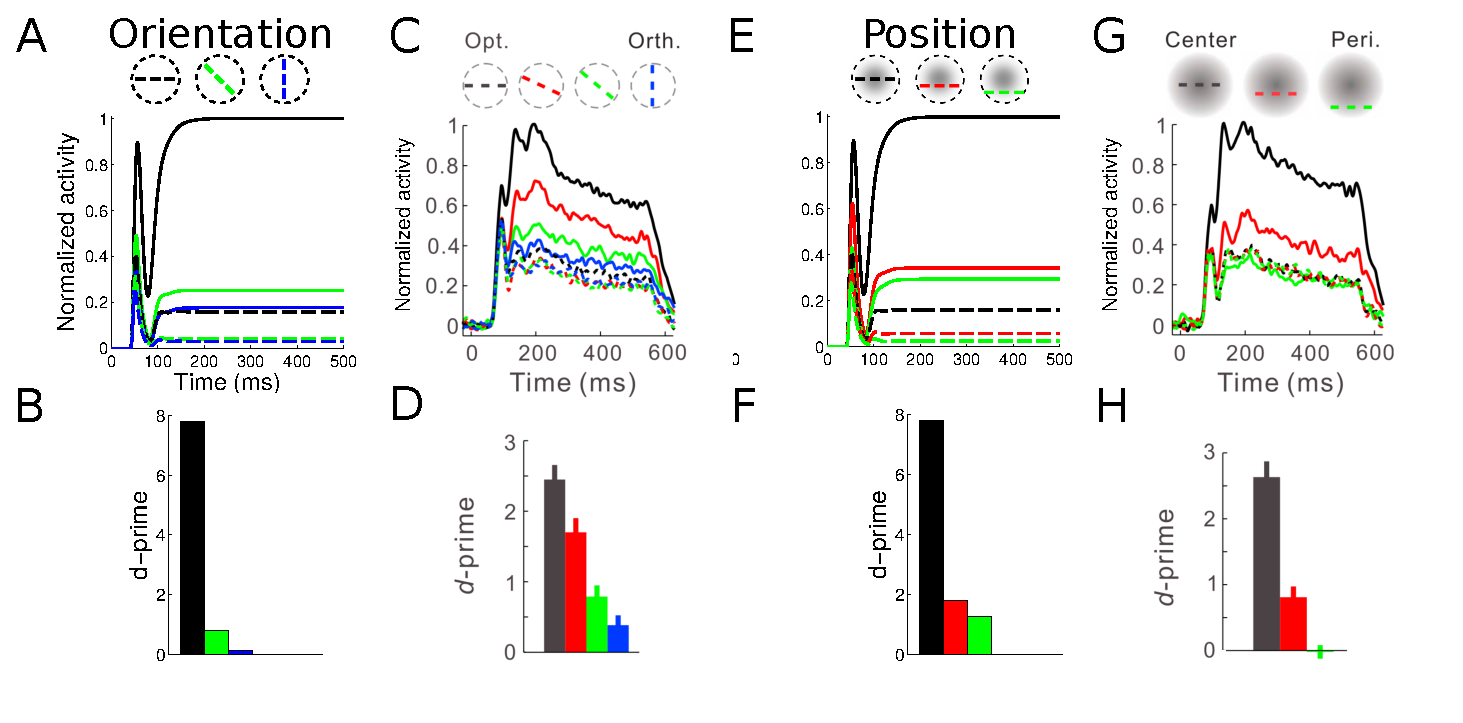
\includegraphics[width=0.75\textwidth]{FigS1.eps}
\end{center}
\caption{Orientation and position dependence of contour integration in
  V4 $G_c$ cells. The top row shows neuronal responses and the bottom
  row the contour-response $d'$.  Line colors for each figure are
  indicated by the legends at the top of each column. Top row, solid
  lines indicate responses for the 7-bar contour pattern, while dashed
  lines indicate responses for the 1-bar (noise)
 pattern.  Note that orientations were changed in variable steps based on the tuning
  curve of the neuron under study in the experimental data
  (panels~C,~D) while our simulation only allowed steps of
  $\pi/4$ (panels~A,B).  (A and B) Model results, orientation
  dependence.
 The neuronal responses (A) and the contour-response $d'$
  (B) decreased when the contour was rotated away from the preferred
  orientation. (C and D) Analogous experimental results, adapted from
  \cite{Chen_etal14}.
  (E and F) Model
  results, position dependence.
 The neuronal responses (E) and
  contour-response $d'$ (F) decreased when the contour was translated
  away from the center of the V4 RF. (G and H) Analogous experimental
  results, adapted from \cite{Chen_etal14}.
  Panels C, D, G, and H are modified from Figure~3 of~\cite{Chen_etal14}.}
\label{Fig:V4_total}
\end{figure*}
%en I forgot, did you get permission from the publishers for
%reproducing their figures? Even if they are modified, may be a good
%idea to be on the safe side.
%
%bh I didn't get permission, since we'll have to pay for each figure, even though we didn't end up
%actually reproducing the entire figure in full. I thought the conclusion we came
%to last time after discussing is to reference the figures in each caption, but
%since we didn't reproduce the whole figure in full, but essentially only the necessary
%panels, we wouldn't request permission from the editor. Please advise.
%
%The affected figures are:
%
%1) Figure 4, we use two panels from Chen et al, 14 (their Figure 2 A,F)
%2) Figure 9, we use one panel from Qiu et al, 07 (their Figure 3 D)
%3) Figure S1, we use four panels from Chen et al, 14 (their Figure 3 A,C,E,G)
%en OK, I think this will be fine.
%
\begin{figure*}[t]
\begin{center}
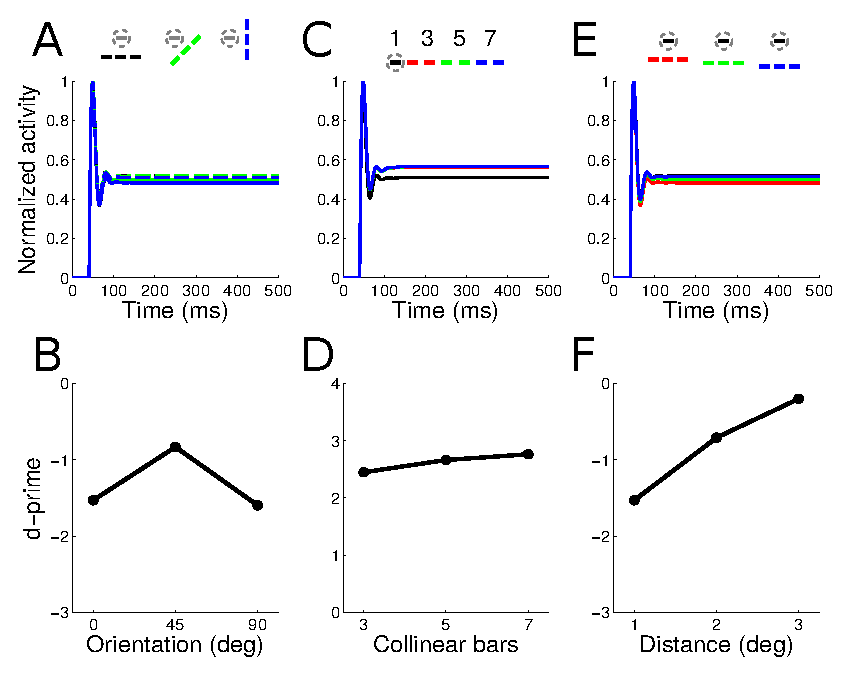
\includegraphics[width=0.75\textwidth]{FigS2.eps}
\end{center}
\caption{Orientation and position dependence of contour integration in
  V1 $E$ cells, model results. The top row shows neuronal responses
  and the bottom row the contour-response $d'$. Line colors for each
  figures are indicated by the legends at the top of each column. (A
  and B) Orientation dependence of background suppression. The
  neuronal responses (A) and the contour-response $d'$ (B) increased
  for intermediate orientations of the background contour.
  In (A), solid and dashed lines correspond to the 7-bar contour and 1-bar noise patterns, respectively.
  (C and D) Contour integration on one end. The neuronal responses (C)
  and contour-response $d'$ (D) increased when bars were added to only
  one side of the V1 RF. (E and F) Position dependence of background
  suppression.  The neuronal responses (E) and contour-response $d'$
  (F) increased (approached zero) when the background contour was
  moved away from the center of the V1 RF.}
\label{Fig:V1_total}
\end{figure*}

\clearpage
\begin{figure*}[t]
\begin{center}
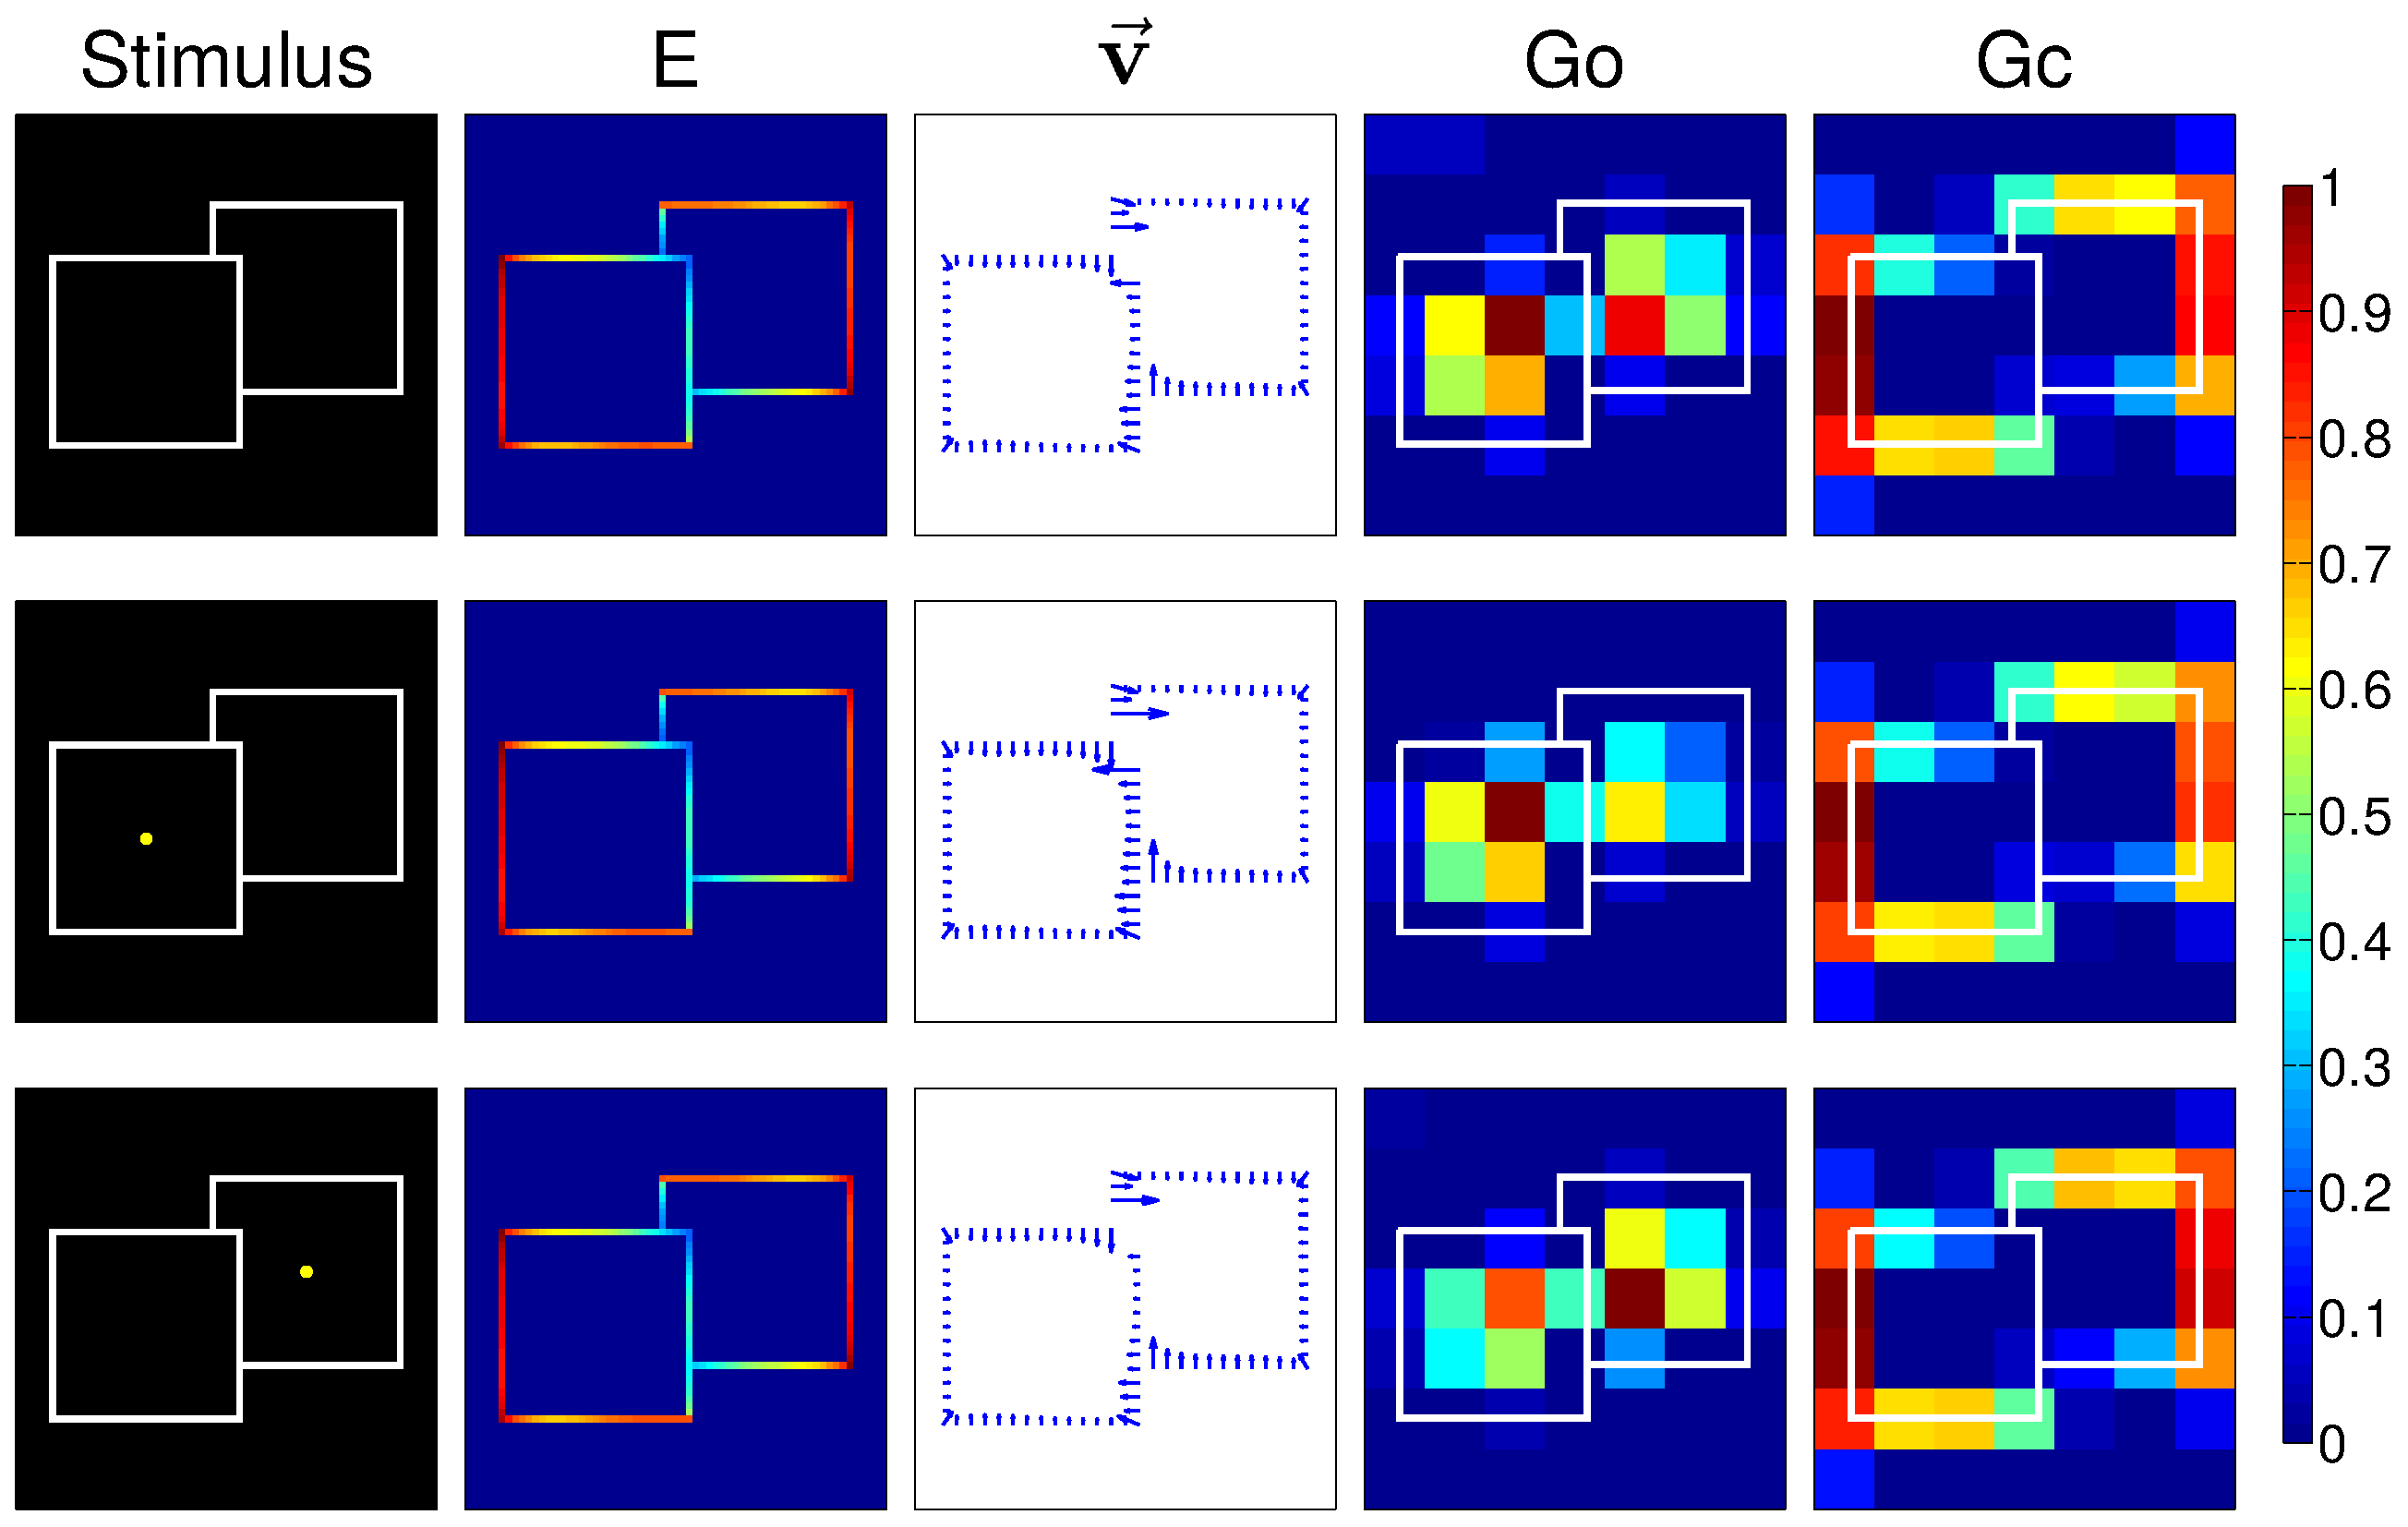
\includegraphics[width=0.75\textwidth]{FigS3.eps}
\end{center}
\caption{Attention in the presence of multiple objects. Shown are
  (left to right) the input stimulus, the edge cell activity (E), the
  border ownership assignment along edges (shown as the vector
  modulation index 
  $\protect\vv{\mathbf{v}}$,
   section~\ref{sec:vmi}), the object
  grouping neuron activity (Go), and the contour grouping activity
  (Gc). 
  The input stimulus is overlaid (white lines) on top of the grouping
  cell activities (columns 4 and~5) to aid visualizing the location of the
two figures.
  Activities are normalized within each map, and warmer colors
  indicate higher activity (see color bar at right). The yellow dot indicates the locus of attention, which was applied at the level of grouping neurons. In
  the absence of attention (top row) or when attention is directed to
  the foreground square (middle row), the edge between the figures is
  correctly assigned to the foreground. If attention is directed
  toward the background square (bottom row), the border ownership
  signal of this edge is greatly reduced, consistent with experimental
  observations~\citep{Qiu_etal07}.}
\label{Fig:Overlap_Square}
\end{figure*}

Even in the absence of attention, figure-ground segregation can be
observed in the border-ownership assignment along the edges of the two
squares, as well as in the object and contour grouping cell activity
(Figure~\ref{Fig:Overlap_Square}, row 1).  Figure
\ref{Fig:Overlap_Square} shows the responses of different populations
of neurons in our model for the different attention conditions. This
figure should be compared with Figure~3 in
\cite{Mihalas_etal11b} which is a model related to ours but which does
not contain $G_c$ cells. The figure shows that the approximate locations of the
foreground and background squares are represented by two peaks in the
activity of object grouping neurons (fourth column). Selectively
attending to one object enhances the activity of grouping neurons
corresponding to the attended object while simultaneously suppressing
the activity of grouping neurons representing the unattended
object. Attentional modulation at the grouping neuron level is then
propagated back to border-ownership selective neurons along object
boundaries via the feedback grouping circuitry of our model.  Of
particular interest is the center edge separating the foreground and
background squares. When attention is directed to the foreground
square, assignment of border ownership along this edge is strengthened
relative to the unattended case (Figure~\ref{Fig:Overlap_Square}, row
2).  However, if attention is directed toward the background square,
border-ownership modulation of the edge between the two squares is
greatly reduced (Figure~\ref{Fig:Overlap_Square}, row 3).  These
results are in agreement with the physiological
evidence~\citep{Qiu_etal07}, and demonstrate that grouping mechanisms
provide a means to attend to objects in clutter.  Functionally, when
attention is directed towards the occluded object, suppression of the
border-ownership signal along the occluding edge is useful because
this edge is ``owned'' by the occluder and should not be included in
the representation of the attended object~\citep{Craft_etal07}.




\clearpage

\end{document}
% end of file template.tex

